\documentclass[11pt,a4paper]{article}

\usepackage[margin=2.35cm]{geometry}
\usepackage[T1]{fontenc}
\usepackage[utf8]{inputenc}
\usepackage{lmodern}
\usepackage{microtype}
\usepackage{graphicx}
\usepackage{booktabs}
\usepackage{tabularx}
\usepackage{longtable}
\usepackage{amsmath}
\usepackage{xcolor}
\usepackage[hidelinks]{hyperref}
\usepackage{float}
\usepackage{caption}
\usepackage{subcaption}

\graphicspath{{../reports/2026-09/}{../experiments/2026-09/}{../robustness/2026-09/}}
\setlength{\parindent}{0pt}
\setlength{\parskip}{0.55em}
\newcommand{\code}[1]{\texttt{#1}}

\title{Fair and Constraint-Aware Radiology Shift Scheduling:\\
A Computational Perspective on Fairness, Robustness and Explainability}
\author{Joana Pimenta\\University of Bologna --- Master in Artificial Intelligence\\
\href{mailto:joana.monteiro@studio.unibo.it}{joana.monteiro@studio.unibo.it}}
\date{September 2026}

\begin{document}
\maketitle

\begin{center}
\begin{tabular}{rl}
Name: & Joana \\
Surname: & Pimenta \\
University email: & \href{mailto:joana.monteiro@studio.unibo.it}{joana.monteiro@studio.unibo.it} \\
Matricola: & \textbf{1168774}
\end{tabular}
\end{center}

\begin{abstract}
This project develops and evaluates a decision-support system for monthly shift scheduling of radiology technicians at Hospital da Covilh\~a, Portugal. The scheduling process is characterised by minimum coverage requirements, heterogeneous shift eligibility, vacations and other absences, working-time limits, rest rules, schedule-pattern preferences and fairness obligations that are carried across months. The system formalises these requirements as a constraint optimisation problem and solves it with the CP-SAT solver. Hard constraints encode conditions that must not be violated; weighted soft constraints represent preferences and operational compromises. The evaluation addresses three dimensions of Trustworthy AI. Fairness is assessed through raw and availability-normalised workload, night and weekend burdens, Gini coefficients and Jain indices, complemented by four alternative objective profiles compared with the published schedule. Robustness is evaluated in six controlled disruption scenarios, all of which produced feasible repairs requiring between two and 12 assignment edits. Explainability is implemented as concrete checks: direct reasons why a worker could not receive a shift, exact changes after a disruption, and new solver runs that test alternative assignments and staffing levels. The September 2026 schedule enforces a mandatory minimum of six Imaging workers on every weekday morning, uses 331 overtime hours, and remains below the preferred target of 10 on nine days. The published gaps total 24 worker-slots. A separate optimisation proves that at least 17 missing worker-slots are unavoidable under the encoded constraints; the returned minimum-gap schedule uses 384 overtime hours. The system is therefore presented as an auditable assistant for human schedulers, not an autonomous authority.
\end{abstract}

\tableofcontents
\newpage

\section{Introduction}
Monthly hospital scheduling is a high-impact allocation problem because it distributes paid work, nights, weekends, inconvenient sequences and rest days among employees while also determining whether a clinical service has adequate staff. Hospital rostering is a well-established but difficult personnel-scheduling problem in which service requirements, workload balance and working conditions interact \cite{burke}. Ethical considerations are therefore important both for protecting the population served by the hospital and for maintaining a fair balance among employees. Workers should not be excessively burdened with undesirable shifts, but should have equitable access to higher-paid duties, within applicable working-time limits and with adequate opportunities for rest \cite{workingtime}.

The problem becomes particularly difficult when ordinary contractual capacity is insufficient to meet demand. Overtime must then be allocated, which necessarily means that some employees will work more hours than others. In a manual process, decisions about who receives this additional burden may be influenced, or be perceived as being influenced, by personal relationships or inconsistent judgement. A constraint solver offers procedural consistency by applying the same encoded rules to every eligible worker. This can support a fairer process and reduce room for ad hoc favouritism. It does not, however, make the result automatically fair, because the solver still implements human choices about inputs, constraints and priorities. Fairness must therefore be treated as a property of the wider sociotechnical process, not merely of the optimisation algorithm \cite{selbst}.

This project was developed in collaboration with the Radiology Service at Hospital da Covilhã. It adapts the course proposal on fair and constraint-aware shift scheduling to a real-world case study by incorporating operational constraints provided by hospital staff. Its objective is not only to produce a timetable, but also to make the assumptions, compromises and consequences of that timetable visible. The main research question is:

\begin{quote}
How can operational feasibility, worker fairness, resilience to disruption, and understandable justification be represented and evaluated in one scheduling decision-support system?
\end{quote}

The work makes four contributions:

\begin{itemize}
  \item a configurable constraint model that distinguishes mandatory rules from weighted preferences;
  \item worker-level and aggregate fairness evaluation, including normalisation by opportunity;
  \item controlled robustness tests that quantify repair feasibility and schedule instability;
  \item factual, local, repair and counterfactual explanations with explicit epistemic limits.
\end{itemize}

The September 2026 configuration is the principal case study. It contains 21 Imaging workers, 30 calendar days, worker-specific vacation periods, consultation assignments, sick leave, contract data, carried rest and rotation histories. A smaller Hemodynamics sub-schedule is also supported. The case-study data were supplied by the Radiology Service, and their use for this academic project was authorised by the hospital. This project-specific authorisation should not be interpreted as permission for unrelated reuse or wider disclosure of the underlying personnel data.

\section{Problem Definition}

\subsection{Service and workforce}

The task is to construct one monthly roster for two connected units of the Radiology Service: Imaging and Hemodynamics. The September 2026 Imaging configuration contains 21 workers while Hemodynamics has three possible workers: Angelo, Nuno and Lina. Angelo and Nuno are dedicated to Hemodynamics, whereas Lina is shared with Imaging, for a total of 23 distinct workers across the two units.

The two schedules cannot be produced independently because Lina cannot work in both departments on the same day. The system first determines the Hemodynamics schedule, where the small team gives it less flexibility. Every day assigned to Lina in Hemodynamics is then blocked in her Imaging schedule, and her Hemodynamics hours reduce her remaining monthly capacity in Imaging. This creates a direct connection between decisions made in the two units.

\subsection{Planning period and worker information}

The planning horizon is one calendar month. For each worker, the system may use:

\begin{itemize}
  \item department membership and eligibility for each shift type;
  \item vacation, sick-leave and consultation dates;
  \item a 35- or 40-hour weekly contract;
  \item rest hours carried into the month;
  \item the final assignment of the preceding month, so that boundary rest rules are respected;
  \item cumulative workday and public-holiday histories, used to rotate future burdens.
\end{itemize}

The required output is a complete monthly allocation identifying who works in each department, on which date and in which shift or duty. A valid schedule must satisfy all mandatory coverage, availability, eligibility, working-time and rest constraints.

\subsection{Imaging shifts}

Table~\ref{tab:problem-shifts} lists the four Imaging shift types. All shifts count as eight working hours. The early-afternoon shift is a special time variant of the afternoon category rather than a fourth independent coverage category.

\begin{table}[H]
\centering
\caption{Imaging shift types.}
\label{tab:problem-shifts}
\begin{tabular}{lll}
\toprule
Code & Time & Meaning \\
\midrule
M & 08:00--16:00 & Morning \\
A & 16:00--00:00 & Normal afternoon \\
EA & 14:00--22:00 & Early-afternoon variant \\
N & 00:00--08:00 & Night \\
\bottomrule
\end{tabular}
\end{table}

Eligibility is heterogeneous. Some workers can perform all three main shift categories, while others cannot work nights; Celia is morning-only and Celso is limited to weekday mornings and afternoons. These eligibility rules are combined with each worker's absences before assignments are created.

\subsection{Imaging staffing requirements}

Table~\ref{tab:problem-coverage} states the implemented staffing levels. Ordinary weekdays distinguish a mandatory morning floor of six from a preferred target of 10. The solver may return between six and 10 morning workers without violating a hard constraint, but every missing worker relative to 10 is reported and penalised. Eleven is the weekday-morning maximum. The afternoon and night numbers, and all weekend or public-holiday numbers, are mandatory minima.

\begin{table}[H]
\centering
\caption{Imaging staffing requirements.}
\label{tab:problem-coverage}
\begin{tabularx}{\textwidth}{Xccc}
\toprule
Day type & Morning & Afternoon & Night \\
\midrule
Ordinary weekday & Minimum 6; preferred 10; maximum 11 & Minimum 3 & Minimum 1 \\
Weekend or public holiday & Minimum 4 & Minimum 2 & Minimum 1 \\
\bottomrule
\end{tabularx}
\end{table}

Exactly one afternoon worker on every ordinary weekday is assigned the early 14:00--22:00 variant. The remaining afternoon workers use the normal 16:00--00:00 shift. Staffing below the preferred target of 10 morning workers is not a hard-constraint violation, but it is an operational compromise that is reported and penalised. Staffing below the mandatory floor of six would make an ordinary weekday schedule invalid.

\subsection{Hemodynamics}

The Hemodynamics unit has a separate weekday-morning schedule involving Angelo, Nuno and Lina. Exactly two of these three workers must be present every weekday morning. The worker holding prevention duty must also work that morning. If only one of Angelo and Nuno works the morning, Lina supplies the second position; if both Angelo and Nuno work, Lina is not required. The model prefers Thursday when a weekday must have only one of the two dedicated workers, but this is a preference rather than a mandatory rule.

In addition to its weekday morning shifts, the Hemodynamics unit assigns prevention duty. This is an on-call responsibility and is modelled separately from an ordinary eight-hour shift. Exactly one of Angelo and Nuno holds prevention duty on every calendar day. Friday, Saturday and Sunday form one continuous duty block held by the same person. Consecutive blocks alternate when both workers are available for both complete blocks. When one worker is on vacation, the other may continue covering prevention because alternation is then impossible.

A prevention duty on a Sunday or public holiday earns one compensatory rest day. The model reserves a distinct available weekday for each such duty by limiting the number of Hemodynamics mornings that the worker may perform. Prevention duty is not added to ordinary shift hours as an eight-hour assignment; its compensatory-rest consequence is represented explicitly instead.

\subsection{Scheduling objective}

The primary requirement is feasibility: no improvement in a preference can compensate for breaking a mandatory rule. Among feasible schedules, the Imaging model aims to distribute cumulative work and opportunity-adjusted workload fairly, approach the preferred weekday-morning staffing target, reduce overtime, avoid undesirable sequences of work and rest, prepare workers appropriately before nights and rotate weekends and public holidays. When an existing schedule is repaired, it also attempts to preserve as many published assignments as possible.

\section{Implementation Technologies}

\subsection{Python and OR-Tools CP-SAT}

The implementation is written in Python. The scheduling model uses Google OR-Tools CP-SAT, a constraint-programming solver for integer and Boolean models \cite{ortools}. CP-SAT is appropriate because shift assignments are discrete, many rules are logical or cardinality constraints, and the objective is a weighted sum of penalties. Under a time limit, it can return a feasible solution together with an objective bound; a \textsc{Feasible} status does not itself certify optimality \cite{ortools}.

\subsection{Data and reporting stack}

Inputs and outputs use JSON and CSV so that assumptions and schedules can be inspected without specialised software. Matplotlib and NumPy are also used to generate timetable, fairness, trade-off, staffing, overtime, and robustness figures. The implementation is divided into the solver (\code{solver.py}), fairness evaluator (\code{evaluate.py}), experiment runner (\code{experiments.py}), robustness suite (\code{robustness.py}), explanation generator (\code{explanations.py}), and visual reporting utilities.

\section{Scheduling System}

\subsection{Inputs and outputs}

For a selected month, the system reads the provided roster, vacations, consultations, sick leave, contract hours, prior-month rest debt, workday history and holiday rotation history. Its primary output is a row-oriented schedule containing date, worker, and shift. It additionally produces compensatory-rest records, prevention duty, fairness metrics, figures, solver diagnostics and carried state for the next month.

Four shift codes appear in the implementation: morning (M, 08:00--16:00), afternoon (A, 16:00--00:00), early afternoon (EA, 14:00--22:00), and night (N, 00:00--08:00). All have eight-hour duration. Eligibility differs by worker: for example, some workers do not work nights, one worker is morning-only and one works weekday mornings or afternoons only.

\subsection{Decision variables}

We define the central Boolean variable as
\[
x_{pds}=\begin{cases}
1 & \text{if worker }p\text{ is assigned to shift }s\text{ on day }d,\\
0 & \text{otherwise.}
\end{cases}
\]
where $P$ is the set of workers, $D$ is the set of dates in the month, and $S=\{M,A,N\}$ is the set of main shift categories.

Additional Boolean and integer variables represent the early-afternoon variant, prevention duty, morning participation, daily morning shortfall, monthly overtime, workload deviations, patterns of consecutive work, and schedule changes during repair.

\subsection{Hard constraints}

The principal rules defined in the model are:

\begin{itemize}
  \item at most one shift per worker and calendar day;
  \item availability and worker-specific shift eligibility;
  \item weekly working time not exceeding 40 hours;
  \item monthly contractual caps adjusted for carried rest, with actual overtime constrained to zero or 24--32 hours per overtime recipient;
  \item no morning immediately after a standard afternoon;
  \item no night immediately after an early afternoon;
  \item no work on the day after a night and minimum spacing between nights;
  \item floor/ceiling sharing of night shifts among eligible workers;
  \item minimum staffing for afternoons and nights, a hard weekday-morning floor of six, and maximum weekday-morning staffing;
  \item hemodynamics-specific prevention alternation, compensatory rest, and morning-presence rules.
\end{itemize}

The appendix provides a detailed explanation and mathematical definition of the implemented constraints.

The weekday-morning requirement has two levels. Six workers are an unconditional hard minimum, while 10 workers remain the preferred operational target. Any gap between six and 10 is represented by a non-negative slack variable. On Monday, Wednesday and Friday, it receives a weight of $10{,}000{,}000$; on Tuesday and Thursday, it receives a weight of 500. This design reflects the operational needs communicated by the hospital and permits transparent prioritisation under limited capacity without ever producing a weekday morning with fewer than six assigned Imaging workers. This distinction is especially important in September 2026 because fewer workers are available.

\subsection{Soft preferences and objective}

Let $c_k(x)$ be the violation count or magnitude for preference $k$ and $w_k$ its configured weight. The solver minimises
\[
\min_x \sum_k w_k c_k(x).
\]

The main-run objective contains the following terms. A larger weight means that one unit of that penalty has a larger effect on the solution, although the numerical scales of the terms also differ.

\begin{itemize}
  \item \textbf{Cumulative workday balance} ($w=100{,}000$): minimises the difference between the largest and smallest cumulative numbers of worked days, including history carried from earlier months.

  \item \textbf{Opportunity-proportional workload deviation} ($w=100$): minimises the largest difference between a worker's assigned hours and the workload expected from their availability. The implementation uses a scaled integer expression to avoid division.

  \item \textbf{Excess work streaks} ($w=500$): penalises every six-day window in which a worker is assigned on all six days. Five consecutive working days are therefore preferred, although the rule remains soft.

  \item \textbf{Isolated work days} ($w=300$): penalises a single working day placed between two rest days.

  \item \textbf{Isolated rest days} ($w=200$): penalises a single rest day placed between two working days, encouraging rest days to occur in groups.

  \item \textbf{Excess afternoon streaks} ($w=400$): penalises three consecutive afternoon assignments. Three are legally permitted by the hard constraints, but sequences of at most two are preferred.

  \item \textbf{Night-preparation mismatch} ($w=150$): penalises a night shift that is not preceded by either of the two preferred three-day preparation patterns defined by the hospital.

  \item \textbf{Night immediately after vacation} ($w=1{,}000$): penalises assigning a night shift on the first day after a worker's vacation.

  \item \textbf{Ordinary public-holiday rotation} ($w=1{,}000$): reduces the difference between workers' cumulative numbers of public holidays worked, including historical assignments.

  \item \textbf{Special-holiday rotation} ($w=2{,}000$): separately balances assignments on Christmas, New Year and Easter using the carried history for each holiday category.

  \item \textbf{Weekend imbalance} ($w=30$): reduces differences in weekend burden after accounting for how many weekends each worker was available to work.

  \item \textbf{Consecutive weekends} ($w=20$): penalises assigning the same worker on two adjacent weekends.

  \item \textbf{Split weekends} ($w=10$): penalises working only one day of a weekend, preferring a complete worked weekend followed by a complete free weekend when possible.

  \item \textbf{Vacation-adjacent weekends} ($w=5$): penalises work on a weekend directly touching a vacation period.

  \item \textbf{Weekday-morning shortfall on Monday, Wednesday and Friday} ($w=10{,}000{,}000$ per missing worker): strongly discourages staffing below the preferred target of 10 on the busiest weekdays. The mandatory floor of six is still enforced separately as a hard constraint.

  \item \textbf{Weekday-morning shortfall on Tuesday and Thursday} ($w=500$ per missing worker): discourages staffing below 10 on these days, but permits this goal to be traded against overtime, workload and schedule-pattern penalties.

  \item \textbf{Monthly overtime} ($w=50$ per overtime hour): discourages hours above monthly contractual capacity. When overtime is used for a worker, the hard constraints require it to fall within the permitted 24--32 hour band.

  \item \textbf{Changes to a published schedule} ($w=0$ in the main run; $w=100{,}000$ during repair and counterfactual runs): penalises every assignment added or removed relative to the reference schedule, keeping a repair as stable as possible.
\end{itemize}

The Hemodynamics model has one additional and separate soft term: a penalty of 300 when only one of Angelo and Nuno works a weekday morning other than Thursday. This makes Thursday the preferred day for Lina to provide the second morning position when such single coverage is necessary.

The weights encode an operational prioritisation and make unlike penalties comparable only through an explicit design choice. For this reason, the system saves both raw and weighted components and compares multiple profiles rather than treating one objective as uniquely correct. Before operational deployment, the weights should be reviewed with hospital schedulers and worker representatives and adjusted in response to identified strengths and shortcomings.

\subsection{Solution workflow}
The system first reads and organises the hospital data, including worker availability, eligibility, contracts and scheduling history. It then builds a mathematical model containing all mandatory rules and weighted preferences. CP-SAT searches for a valid schedule that minimises the objective function, stopping when it proves optimality or reaches the time limit. The resulting schedule is evaluated for staffing coverage, overtime and fairness, after which the program produces the timetable, machine-readable reports, figures and explanations for human review. When an existing schedule must be repaired after a disruption, the original assignments are used as a reference and changes receive a high penalty, encouraging the solver to alter as little of the published schedule as possible.

\begin{figure}[H]
  \centering
  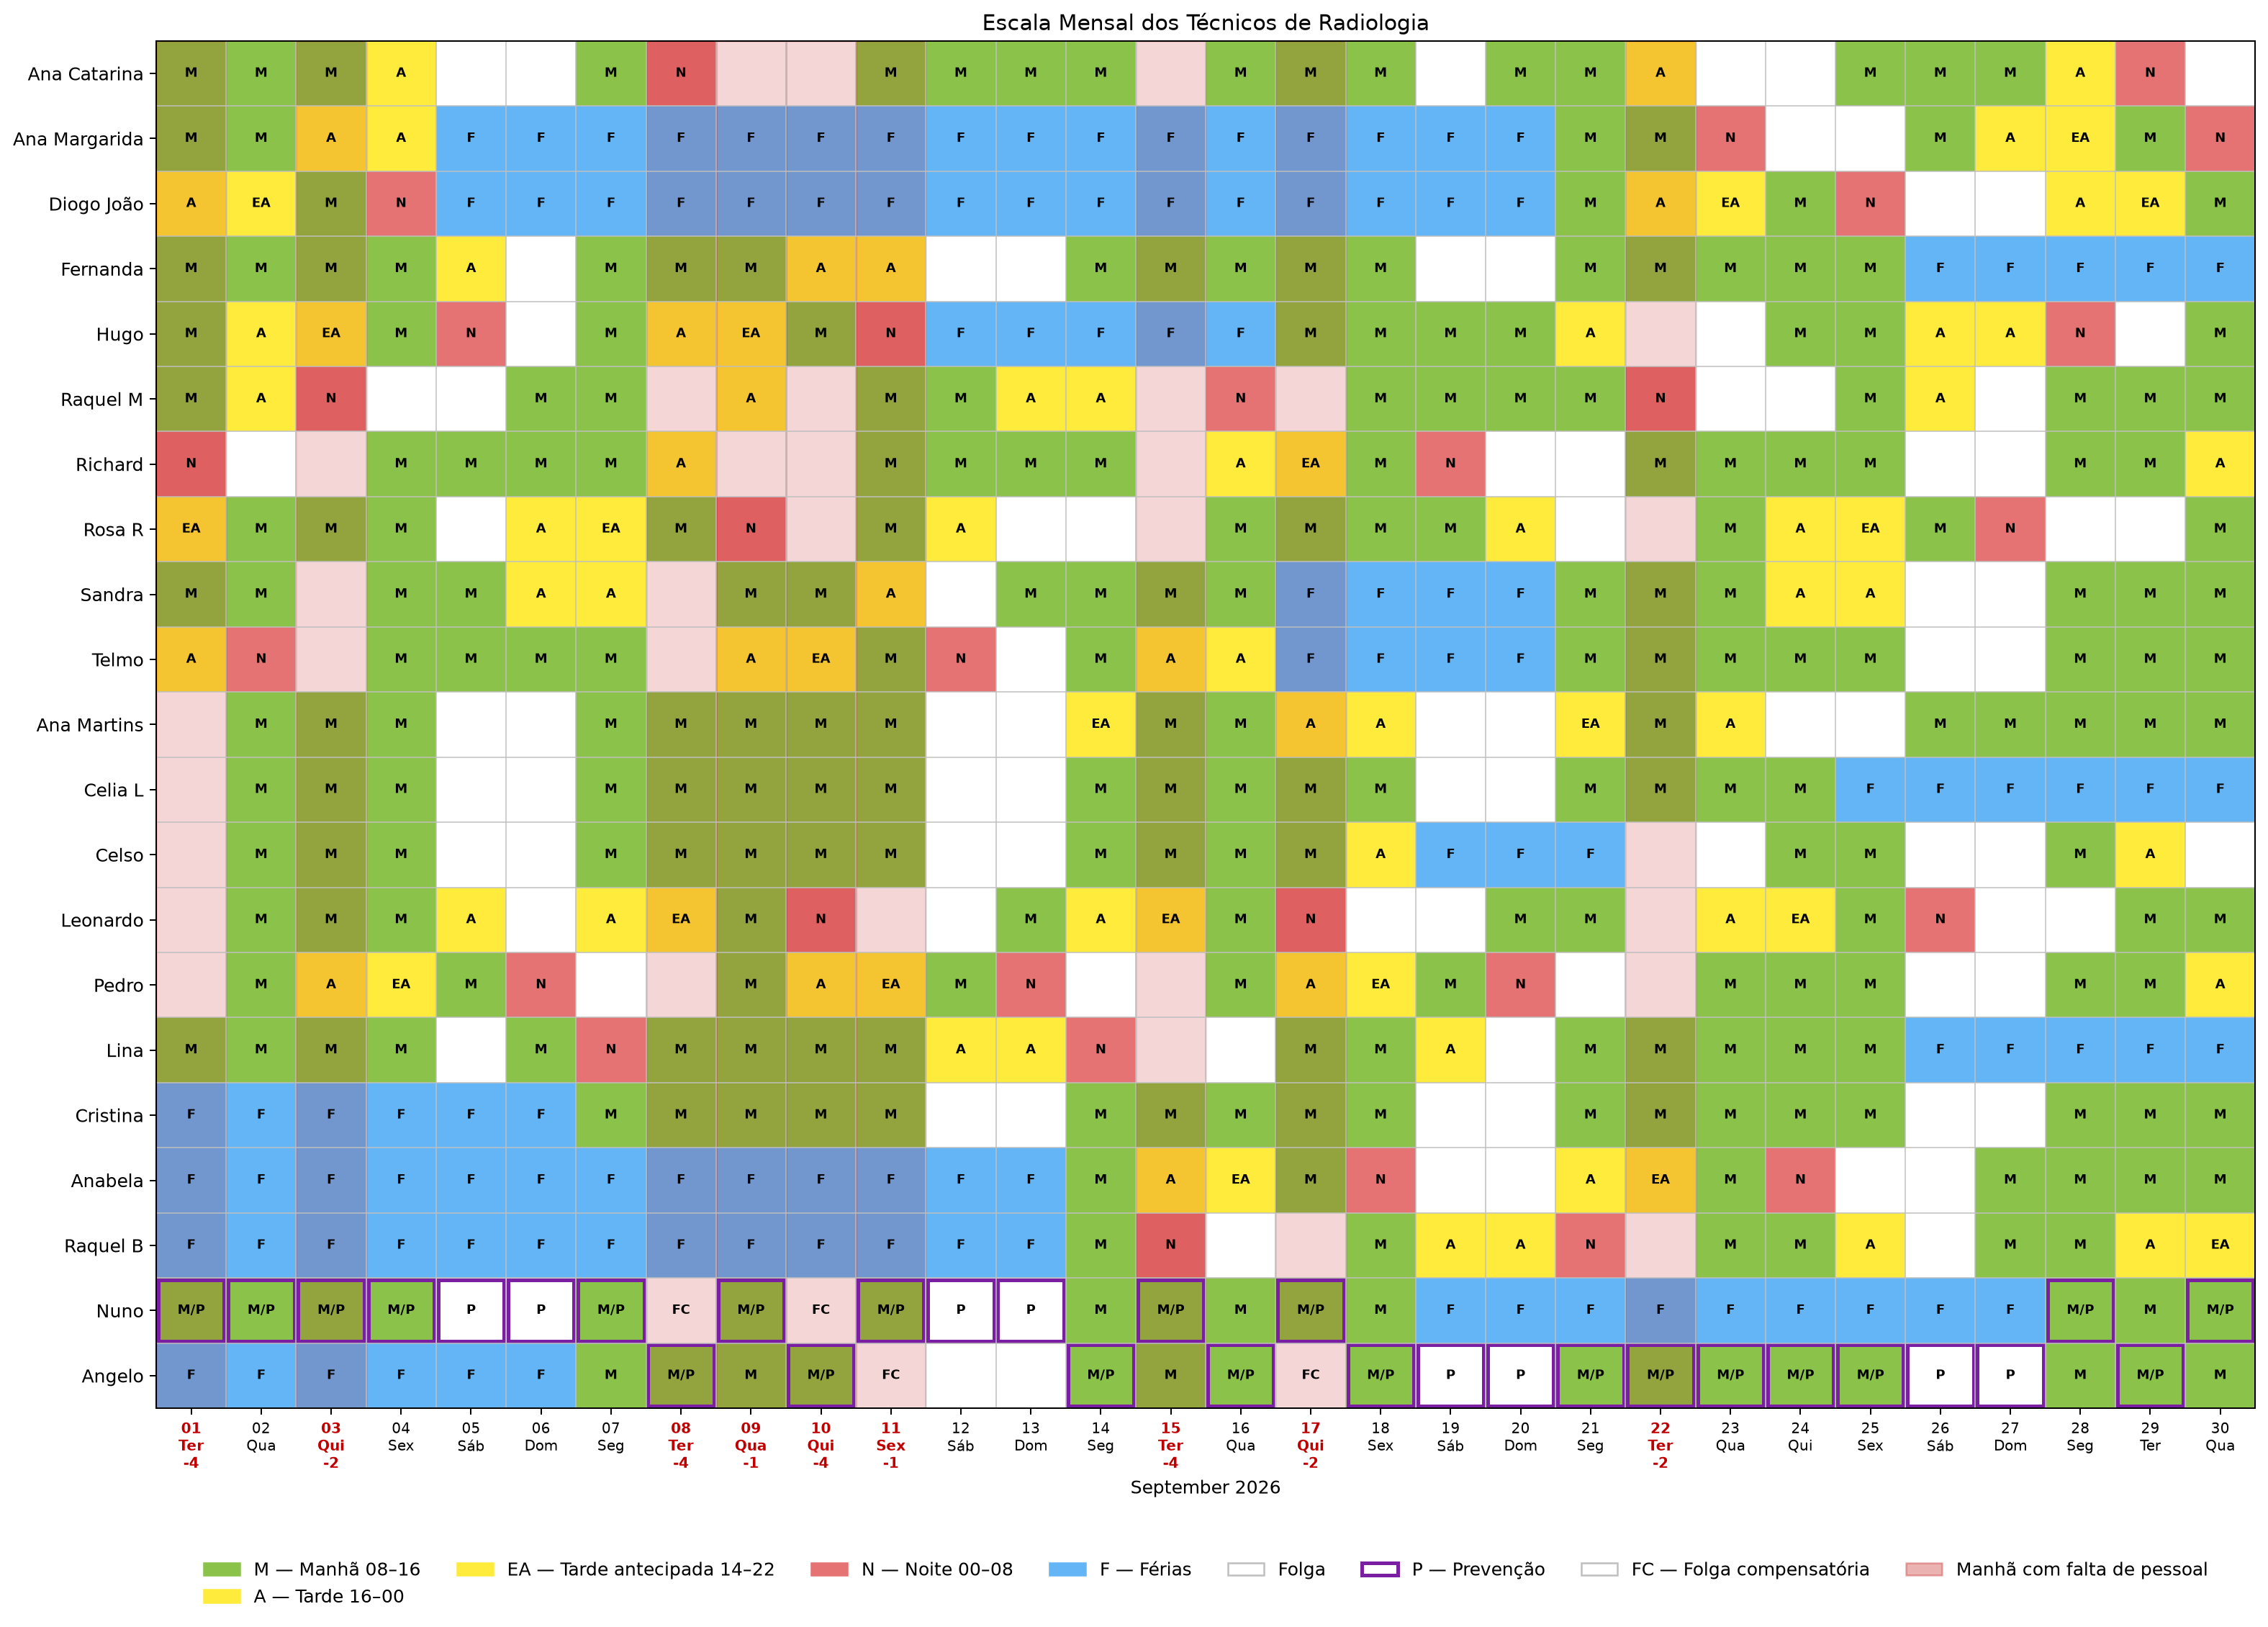
\includegraphics[width=\textwidth]{timetable_combined.png}
  \caption{Generated September 2026 timetable. The figure is an operational review aid; the CSV schedule and solver report are the system's primary outputs.}
  \label{fig:timetable}
\end{figure}

\section{Trustworthy-AI Analysis}

The analysis focuses on fairness, robustness and explainability because these are mutually dependent aspects of trustworthy systems rather than interchangeable scores. This framing follows the European Commission's emphasis on lawful, ethical and robust AI and NIST's treatment of fairness, transparency, explainability, privacy and resilience as contextual, interacting characteristics \cite{euai,nist}.

\subsection{Fairness}

\subsubsection{Fairness targets}

The system considers several distributive goods and burdens: total assigned hours, workload relative to days of availability, nights, nights relative to night opportunities, weekends worked, and weekends relative to available weekends. Opportunity normalisation matters because workers have different vacation periods and shift eligibility. Equal raw night counts, for example, are neither possible nor meaningful when some workers cannot work nights.

For a non-negative vector $y=(y_1,\dots,y_n)$, inequality is measured with the Gini coefficient
\[
G(y)=\frac{\sum_i\sum_j |y_i-y_j|}{2n\sum_i y_i},
\]
where 0 denotes equality \cite{gini}. Jain's index is
\[
J(y)=\frac{(\sum_i y_i)^2}{n\sum_i y_i^2},
\]
where 1 denotes equality \cite{jain}. Both are descriptive summaries, not proofs of justice. Both raw assigned-hours and availability-normalised workload metrics exclude workers with no Imaging opportunity during the month. The denominator of the normalised workload metric also removes Lina's linked Hemodynamics assignments. Normalised night and weekend metrics likewise exclude workers with no opportunity for the corresponding burden.

\subsubsection{Group fairness}

The available worker attributes contain binary sex labels, with 14 female and seven male Imaging workers. Sex is not supplied to the scheduling model and therefore does not influence eligibility, constraints, objective weights or assignment decisions. It is used only after the schedule has been generated to audit whether the two groups experience different outcomes.

The audit examines nights, weekends and public holidays because these are potentially undesirable or inconvenient assignments. Two forms of rate are calculated for each worker. The raw night or weekend rate divides the number of those assignments by the worker's total assigned shifts. The opportunity-normalised rate instead divides by the number of calendar dates on which that worker was statically available and eligible for the relevant assignment. Group values are the means of the available worker-level rates. Workers with no assigned shifts are excluded from raw shift-rate means because their denominator is zero, while workers with no relevant opportunity are excluded from the corresponding opportunity-normalised mean.

For each measure, the audit reports the female mean $r_F$, male mean $r_M$, signed gap $r_F-r_M$, absolute gap $|r_F-r_M|$, and burden ratio $r_F/r_M$. A gap of zero and ratio of one indicate parity for that measure. The overall burden score is the equally weighted mean of each worker's available night, weekend and holiday shift rates. These quantities are descriptive comparisons, not statistical or legal tests of discrimination.

Opportunity is defined statically: a date counts when it is not blocked by vacation, consultation, sick leave or a linked Hemodynamics assignment and the worker profile permits the shift. The calculation does not reconstruct dynamic restrictions created by rest, night spacing, accumulated hours or competition for other shifts. September contains no configured public holiday, so holiday rates are undefined. The audit does not calculate a separate satisfaction score for worker-specific constraints; availability and shift eligibility are instead represented directly in the model and in the opportunity denominators.

\subsection{Fairness--preference trade-off experiments}

Fairness objectives can conflict with one another and with desirable schedule patterns. For example, concentrating work may reduce isolated work days but increase workload inequality, while distributing weekends more equally may require less desirable work sequences. The project therefore does not treat the weights of one objective function as an ethically neutral or uniquely correct choice. It compares the published schedule with four alternative schedules generated from the same September workers, input data and hard constraints. Only the relative importance of soft penalties changes in the four alternatives.

The names of the alternatives describe experimental configurations. In particular, the \emph{operational baseline} is a deliberately simplified comparison profile in which most fairness and schedule-pattern penalties are removed or greatly reduced. The \emph{published schedule} is the main case-study roster generated with the balanced weights and a 600-second solve. It is used directly as the balanced reference here and is also the schedule evaluated throughout the operational, fairness, robustness and explanation results.

\begin{itemize}
  \item \textbf{Operational baseline:} retains the staffing, overtime, afternoon and night-pattern priorities, but gives workday and workload balance weight 1 and disables the general work/rest, holiday and weekend penalties, providing a low fairness priority reference.

  \item \textbf{Workload-focused:} gives cumulative workday balance weight 100,000 and proportional workload deviation weight 1,000. General work/rest penalties receive weight 10, holiday rotation 100/200, and each weekend term weight 1. This profile asks what happens when equality of working hours is prioritised over weekend arrangement and most pattern preferences.

  \item \textbf{Weekend-focused:} gives weekend imbalance weight 1,000, consecutive weekends 250, split weekends 100 and vacation-adjacent weekends 50. Workday balance remains 100,000 and workload deviation 100, while general work/rest penalties receive weight 20. This profile prioritises the distribution and continuity of weekends.

  \item \textbf{Preference-focused:} gives excess work streaks weight 1,000, isolated work and rest days 500 each, holiday rotation 1,000/2,000, and weekend penalties 100--200. It tests stronger protection against undesirable schedule patterns.

  \item \textbf{Published schedule:} uses the balanced weights selected for the main model: workday balance 100,000; workload deviation 100; excess work streaks 500; isolated work/rest days 300/200; holiday rotation 1,000/2,000; and weekend penalties between 5 and 30. This is the case-study schedule and is meant to balance all the considerations above to produce a well-rounded schedule.
\end{itemize}

Several priorities are held constant so that the experiment remains operationally meaningful: weekday-morning shortfall has weight 10,000,000 on Monday, Wednesday and Friday and 500 on Tuesday and Thursday; monthly overtime has weight 50; excess afternoon streaks 400; night-preparation mismatch 150; and a night immediately after vacation 1,000.

Each generated schedule is evaluated using the same outcome measures: availability-normalised workload, night-burden and weekend-burden Gini coefficients and Jain indices, together with a common preference cost. The preference cost is the unweighted sum of the raw soft-penalty components, including workload imbalance. It has no unit because it adds heterogeneous quantities such as scaled workload deviation, counts of schedule patterns, missing morning worker-slots and overtime hours. It is therefore only a broad within-study comparison, not a physical quantity. Raw solver-objective values are not compared across profiles because a value calculated with one set of weights is not on the same scale as a value calculated with another. The corresponding results are reported in Section~\ref{sec:tradeoff-results}.

\subsection{Technical robustness}

Robustness is defined here as the capacity to repair a published schedule after a bounded disruption while retaining feasibility and limiting changes imposed on workers. Six scenarios cover one-day absence, absence of a scheduled night worker, three-day absence, simultaneous absences and increased morning or night demand. For each scenario we record status, time, assignment edits, affected workers, shortfall and changes in fairness indices.

We report coverage slack explicitly and preserve the original schedule during repair where possible. A human scheduler remains responsible for deciding whether a shortfall is operationally tolerable, whether staff are available and whether a repaired timetable can be published.

\subsection{Explainability}

The purpose of the explanation component is to help a scheduler or worker inspect a result and ask what would change under an alternative. It does not claim to reveal a hidden reasoning process inside the solver. The counterfactual approach is motivated by the use of concrete alternative outcomes to support understanding and contestation \cite{wachter}. Four questions are addressed:

\begin{enumerate}
  \item \emph{Does an assignment follow the encoded rules?} The report checks availability, shift eligibility, coverage, working hours and relevant rest rules. This is a compliance check.
  \item \emph{Why was another worker not assigned?} The program looks for a direct blocking reason, such as vacation, lack of eligibility, another shift on the same day, required recovery after a night, or an hours limit. If no direct reason is visible, it says that the choice resulted from the overall optimisation.
  \item \emph{What would happen if an assignment changed?} The selected assignment is forbidden and the complete schedule is solved again. The report states whether an alternative exists and lists the resulting assignment changes.
  \item \emph{Why is a morning below the preferred staffing target?} For each affected day, the solver is rerun with 10 morning workers required. A second experiment minimises the total morning gap across the whole month while ignoring all other preferences. Together these tests distinguish an individually avoidable gap from a month-wide capacity limit.
\end{enumerate}

The distinction is important. Showing that an assignment is legal does not show that it was the only possible assignment. A counterfactual provides stronger evidence because the solver actually constructs an alternative, but its conclusion remains conditional on the encoded rules and input data.

\section{Experimental Evaluation}

\subsection{Case-study setup}

The principal case study covers the 30 days of September 2026. The Imaging roster contains 21 workers, of whom 13 are eligible for night shifts and 18 have at least one weekend opportunity. The sex-group audit contains 14 female and seven male workers. As explained in the Problem Definition, Lina is shared with Hemodynamics, while Angelo and Nuno work only in that unit.

Worker availability is unusually restricted during this month. C\'atia is on sick leave for the entire month and Ana Sofia is assigned to consultations throughout the month, so neither is available for the Imaging roster. In addition, multiple workers have worker-specific vacation periods. The experiment also uses each worker's contract hours, carried rest, cumulative workday history and holiday-rotation history. These differences in availability and eligibility are important when interpreting workload, night and weekend distributions.

The published schedule was generated with random seed 42 and a 600-second Imaging time limit. CP-SAT returned a \textsc{Feasible} solution with objective $23{,}227{,}000$ and best bound $23{,}224{,}915$, corresponding to a relative gap of approximately 0.009\%. The published roster is therefore the best feasible solution found in this run but it is not a solver-certified optimum. Separate trade-off, robustness and explanation experiments use their own stated time limits.

\subsection{Operational result}

Most active and available workers receive 21 shifts (168 hours). Workers with long absences receive 12 or 13 shifts, while Lina receives eight Imaging shifts because her 13 Hemodynamics mornings are accounted for separately. The published roster uses 331 overtime hours across 12 workers; every recipient works between 24 and 32 hours above their adjusted monthly base. No excess-work-streak, excess-afternoon-streak or night-after-vacation penalties occur.

No weekday morning has fewer than the hard minimum of six Imaging workers. Nine dates remain below the preferred target of 10, totalling 24 missing worker-slots relative to that target: September 1, 3, 8, 9, 10, 11, 15, 17, and 22. Actual coverage on these dates ranges from six to nine. Figure \ref{fig:capacity} provides an overview of the capacity pressures underlying these shortfalls. Panel (a) shows daily Imaging morning coverage, highlighting the weekday mornings that fall below the preferred target of 10 workers while still satisfying the hard minimum of six. Panel (b) shows the corresponding monthly overtime assigned to each worker relative to the defined fair-share range. The two panels show that the remaining coverage gaps occur despite substantial use of overtime.

The explanation experiment clarifies why these gaps exist. Requiring 10 workers on eight of the nine affected dates produces a valid alternative schedule, requiring between four and 22 assignment edits and affecting between two and seven workers. Friday, 11 September is different: requiring 10 workers on that morning is proven infeasible under the encoded hard constraints, so its one-worker gap is individually unavoidable. A separate optimisation that minimises only the total morning gap proves that providing 10 workers on every weekday morning is impossible. The smallest possible monthly gap is 17 worker-slots. The returned minimum-gap schedule uses 384 overtime hours, compared with 24 missing worker-slots and 331 overtime hours in the published schedule. These results reveal a clear trade-off between improved morning coverage and increased overtime, which should be evaluated with hospital staff to determine the operationally acceptable balance.

\begin{figure}[H]
  \centering
  \begin{subfigure}{0.61\textwidth}
    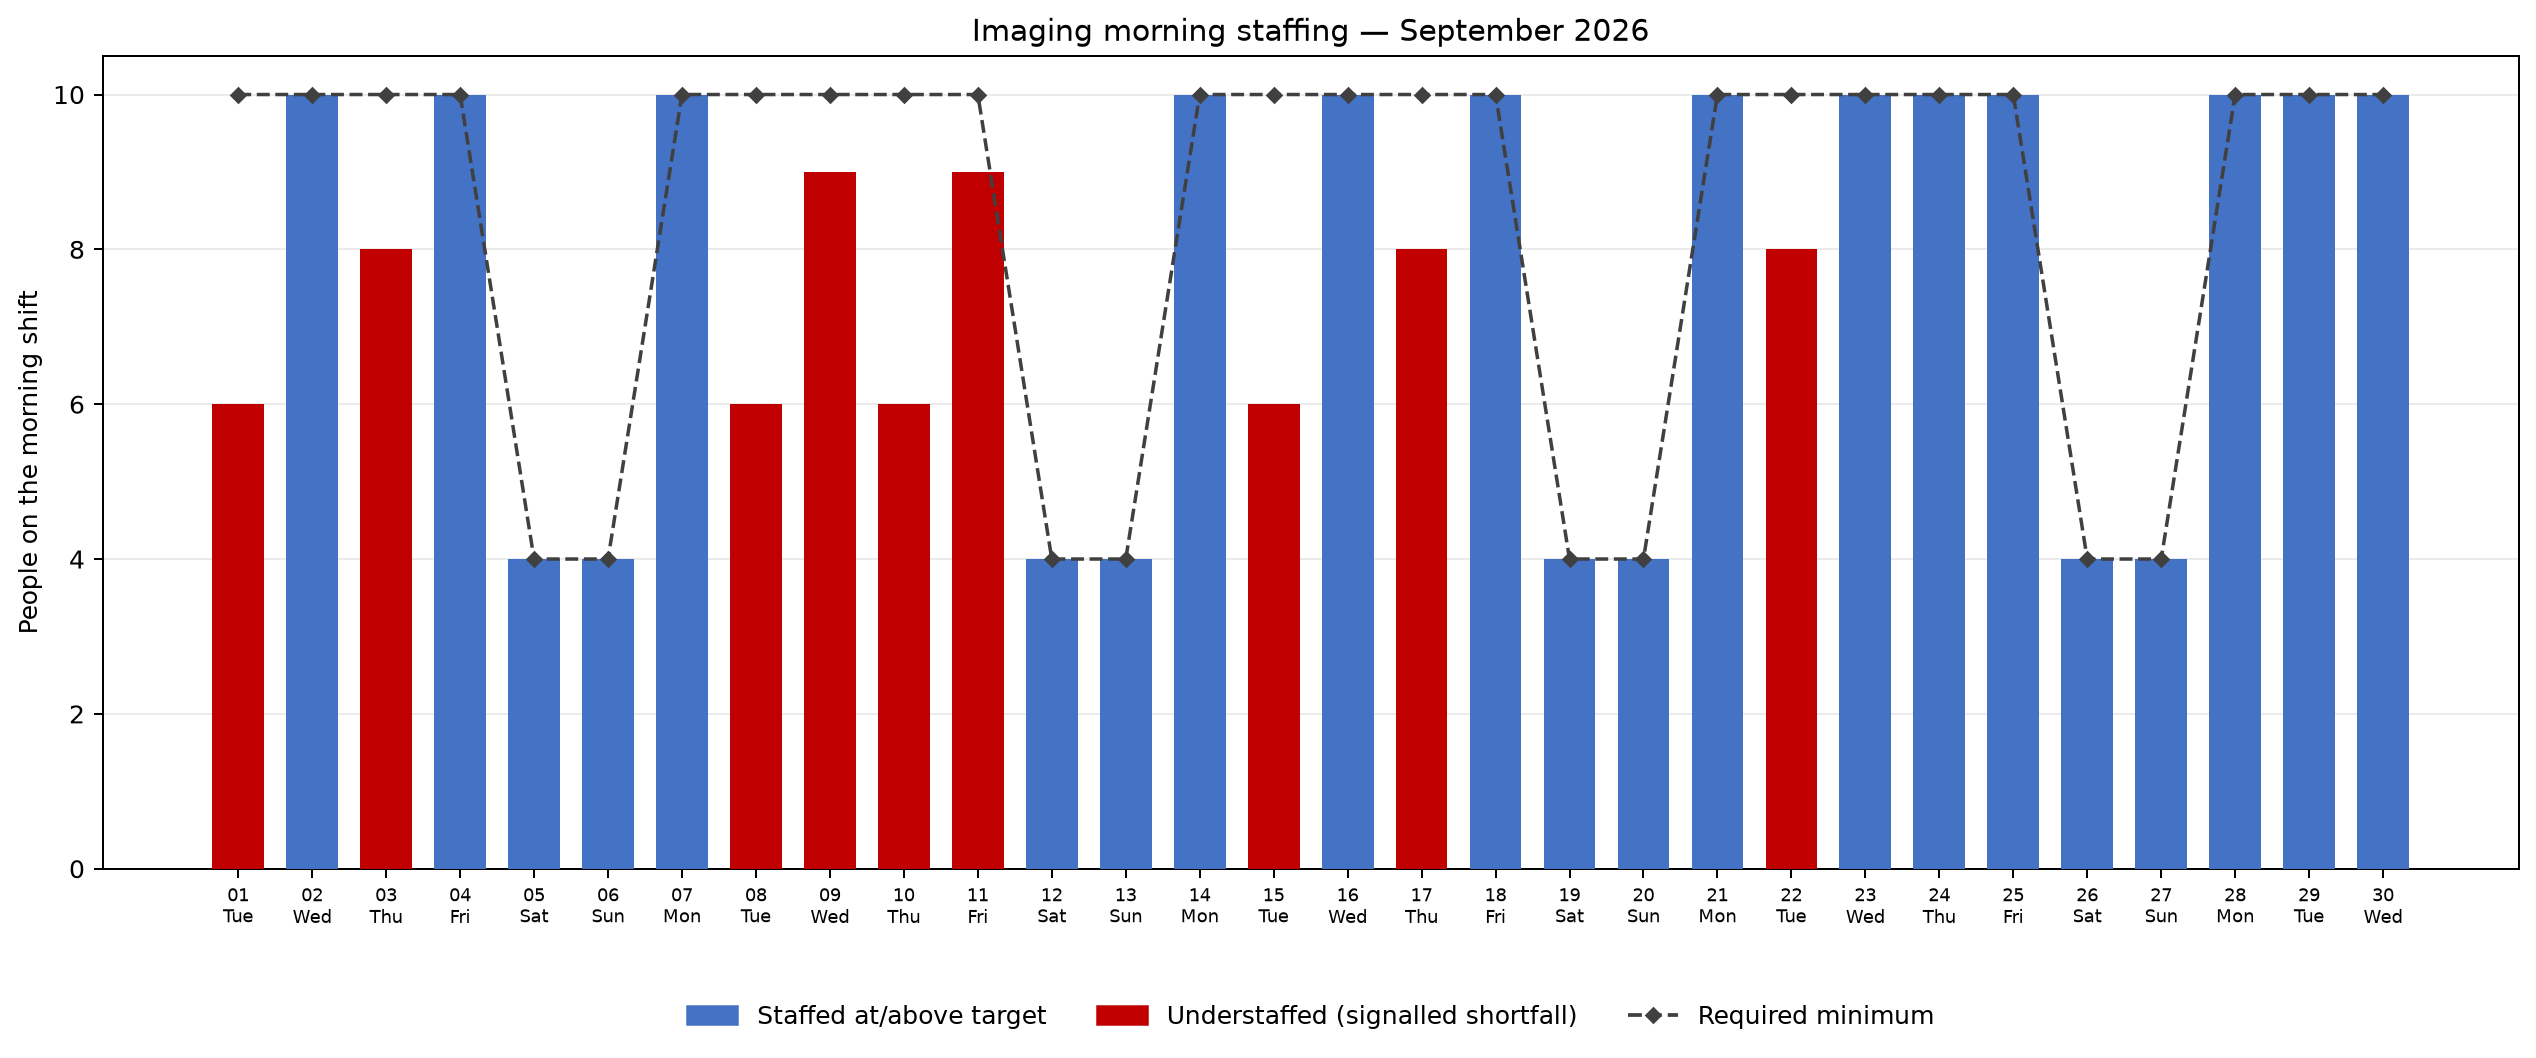
\includegraphics[width=\textwidth]{morning_staffing.png}
    \caption{Morning Imaging coverage and staffing shortfalls.}
  \end{subfigure}
  \hfill
  \begin{subfigure}{0.35\textwidth}
    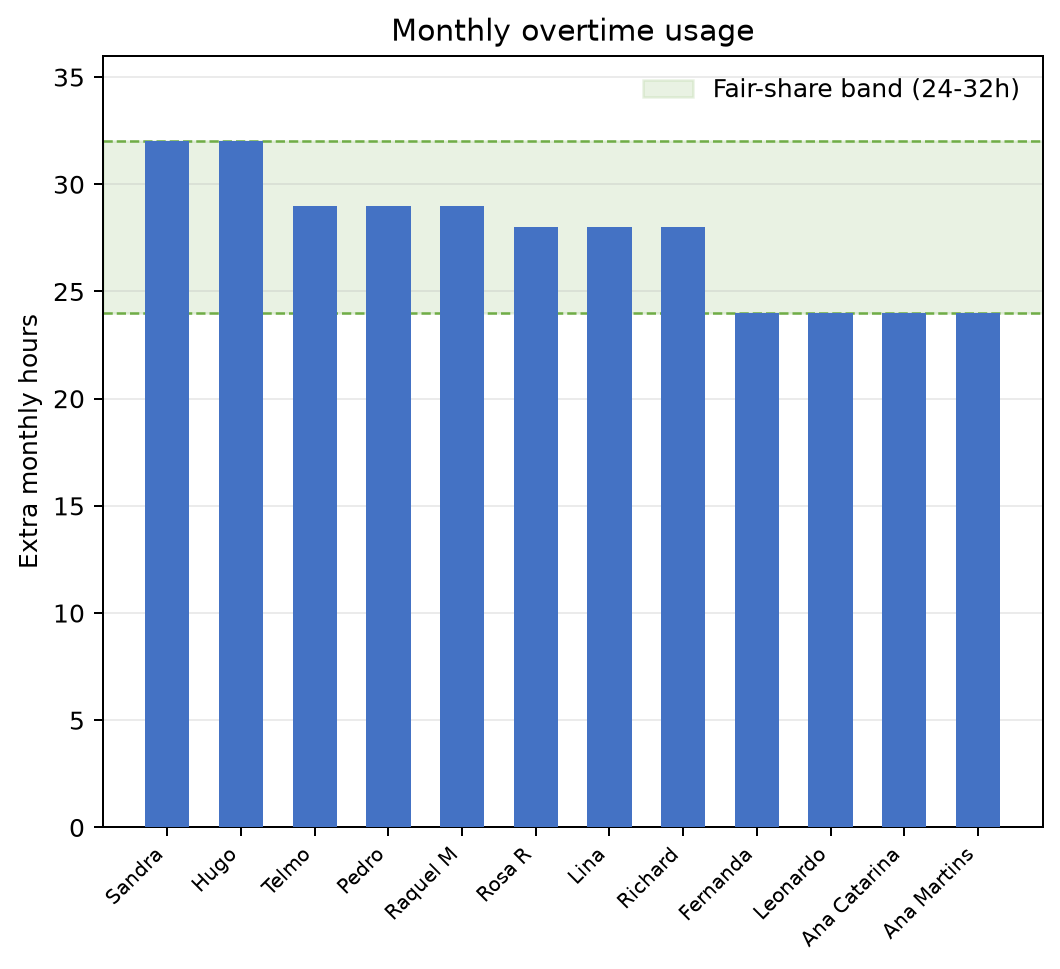
\includegraphics[width=\textwidth]{overtime_usage.png}
    \caption{Distribution of monthly overtime across workers.}
  \end{subfigure}
  \caption{Imaging capacity and overtime diagnostics for the September 2026 schedule. (a) Number of workers assigned to the Imaging morning shift on each day, with weekday mornings below the preferred target of 10 highlighted in red. All weekday assignments satisfy the hard minimum staffing requirement of six workers. (b) Monthly overtime hours assigned to each worker, with the shaded region indicating the 24–32 hour fair-share range.}
  \label{fig:capacity}
\end{figure}

\subsection{Fairness results}

\subsubsection{Individual and distributional results}

Table~\ref{tab:fairness} reports the main fairness results. Night allocation shows that eligible workers receive two or three nights, with coefficients $G=0.0923$ and $J=0.9615$, showing good equality in the raw counts. C\'atia and Ana Sofia are excluded from both workload calculations because neither has an Imaging opportunity during the month. Raw assigned hours remain less equal because several workers have long absences or cross-unit responsibilities. Availability normalisation also removes Lina's Hemodynamics days from her Imaging denominator and shows a much more even workload distribution. Weekend burden remains less even than workload or night burden.

\begin{table}[H]
\centering
\caption{September 2026 fairness metrics.}
\label{tab:fairness}
\begin{tabularx}{\textwidth}{Xrrrrr}
\toprule
Metric & Mean & Min. & Max. & Gini & Jain \\
\midrule
Assigned hours & 143.16 & 64 & 168 & 0.1161 & 0.9504 \\
Availability-normalised workload & 0.7544 & 0.6667 & 0.8571 & 0.0445 & 0.9936 \\
Night shifts (eligible workers) & 2.3077 & 2 & 3 & 0.0923 & 0.9615 \\
Normalised night burden & 0.1065 & 0.0667 & 0.1667 & 0.1631 & 0.9221 \\
Weekends (eligible workers) & 2.0556 & 0 & 4 & 0.3709 & 0.6978 \\
Normalised weekend burden & 0.6482 & 0 & 1 & 0.3079 & 0.7562 \\
\bottomrule
\end{tabularx}
\end{table}

Figure~\ref{fig:fairness} examines fairness from four distinct perspectives: total assigned workload, workload relative to availability, the distribution of night and weekend duties and aggregate equality indices.
The upper-left panel shows raw Imaging workload. Ten workers receive 168 Imaging hours, while workers with substantial absence periods receive fewer. Anabela and Raquel B receive 104 hours, Ana Margarida and Diogo João receive 96, and Cristina receives 144. C\'atia and Ana Sofia receive no Imaging assignments because C\'atia is on sick leave and Ana Sofia is assigned to consultations throughout the month; their zero values remain visible in the chart for context but are excluded from both workload indices and from the displayed mean because neither has an Imaging opportunity. Among the 19 workers included in the workload calculations, Lina receives the minimum of 64 Imaging hours because she also works 13 mornings in Hemodynamics. The mean is 143.16 hours, with an assigned-hours Gini coefficient of 0.1161 and Jain index of 0.9504. Consequently, the remaining raw workload inequality should not be interpreted as evidence that the solver arbitrarily favoured particular workers: much of it is connected to absences and cross-unit responsibilities.
The upper-right panel divides each worker's Imaging assignments by the days on which that worker could participate in Imaging. Cátia and Ana Sofia are excluded from the aggregate because they have no Imaging opportunity. Lina's 13 Hemodynamics mornings are also removed from her denominator, leaving 12 available Imaging days and a ratio of $8/12=0.6667$. Across the 19 workers with at least one opportunity, ratios range from 0.6667 to 0.8571. The resulting Gini coefficient is 0.0445 and the Jain index is 0.9936, showing that availability explains most of the variation in raw Imaging hours.
The lower-left panel separates two undesirable-shift burdens. Night work is distributed relatively evenly among the 13 night-eligible workers: every eligible worker receives either two or three nights. This gives a night-count Gini coefficient of 0.0923 and Jain index of 0.9615. After normalising by static eligible opportunities, the Gini coefficient is 0.1631 and the Jain index is 0.9221. Lina has the largest normalised rate, with two nights across 12 Imaging opportunities, while Rosa, Richard and Ana Catarina each have two nights across 30 opportunities. This shows that equality in the number of nights is not identical to equality relative to opportunity.
Weekend work is less evenly distributed. Eligible workers receive between zero and four distinct worked weekends, producing a weekend-count Gini coefficient of 0.3709 and Jain index of 0.6978. Normalisation by static weekend opportunities improves the result to a Gini coefficient of 0.3079 and Jain index of 0.7562. Raquel B, Rosa, Lina, Hugo, Leonardo, Raquel M and Ana Margarida work every weekend opportunity identified for them, while Celia, Diogo João and Cristina work none of theirs. Ana Martins works one quarter. The schedule therefore distributes workload and night duty more evenly than weekend duty. This does not automatically mean that the weekend allocation is unjust, because eligibility, rest rules and interactions with weekday assignments restrict the available alternatives.
Overall, Figure 3 supports three conclusions. First, raw workload differences are largely explained by vacation, sick leave, consultation duties and Lina's cross-unit role: after those opportunity differences are represented correctly, Imaging workload is highly even. Second, night assignments remain reasonably even, although equality of counts and equality relative to opportunity are not identical. Third, weekend burden is the least evenly distributed outcome and deserves closer examination. The published schedule therefore performs strongly on availability-adjusted workload, reasonably on night equality, but does not achieve equally strong weekend fairness.

\begin{figure}[H]
  \centering
  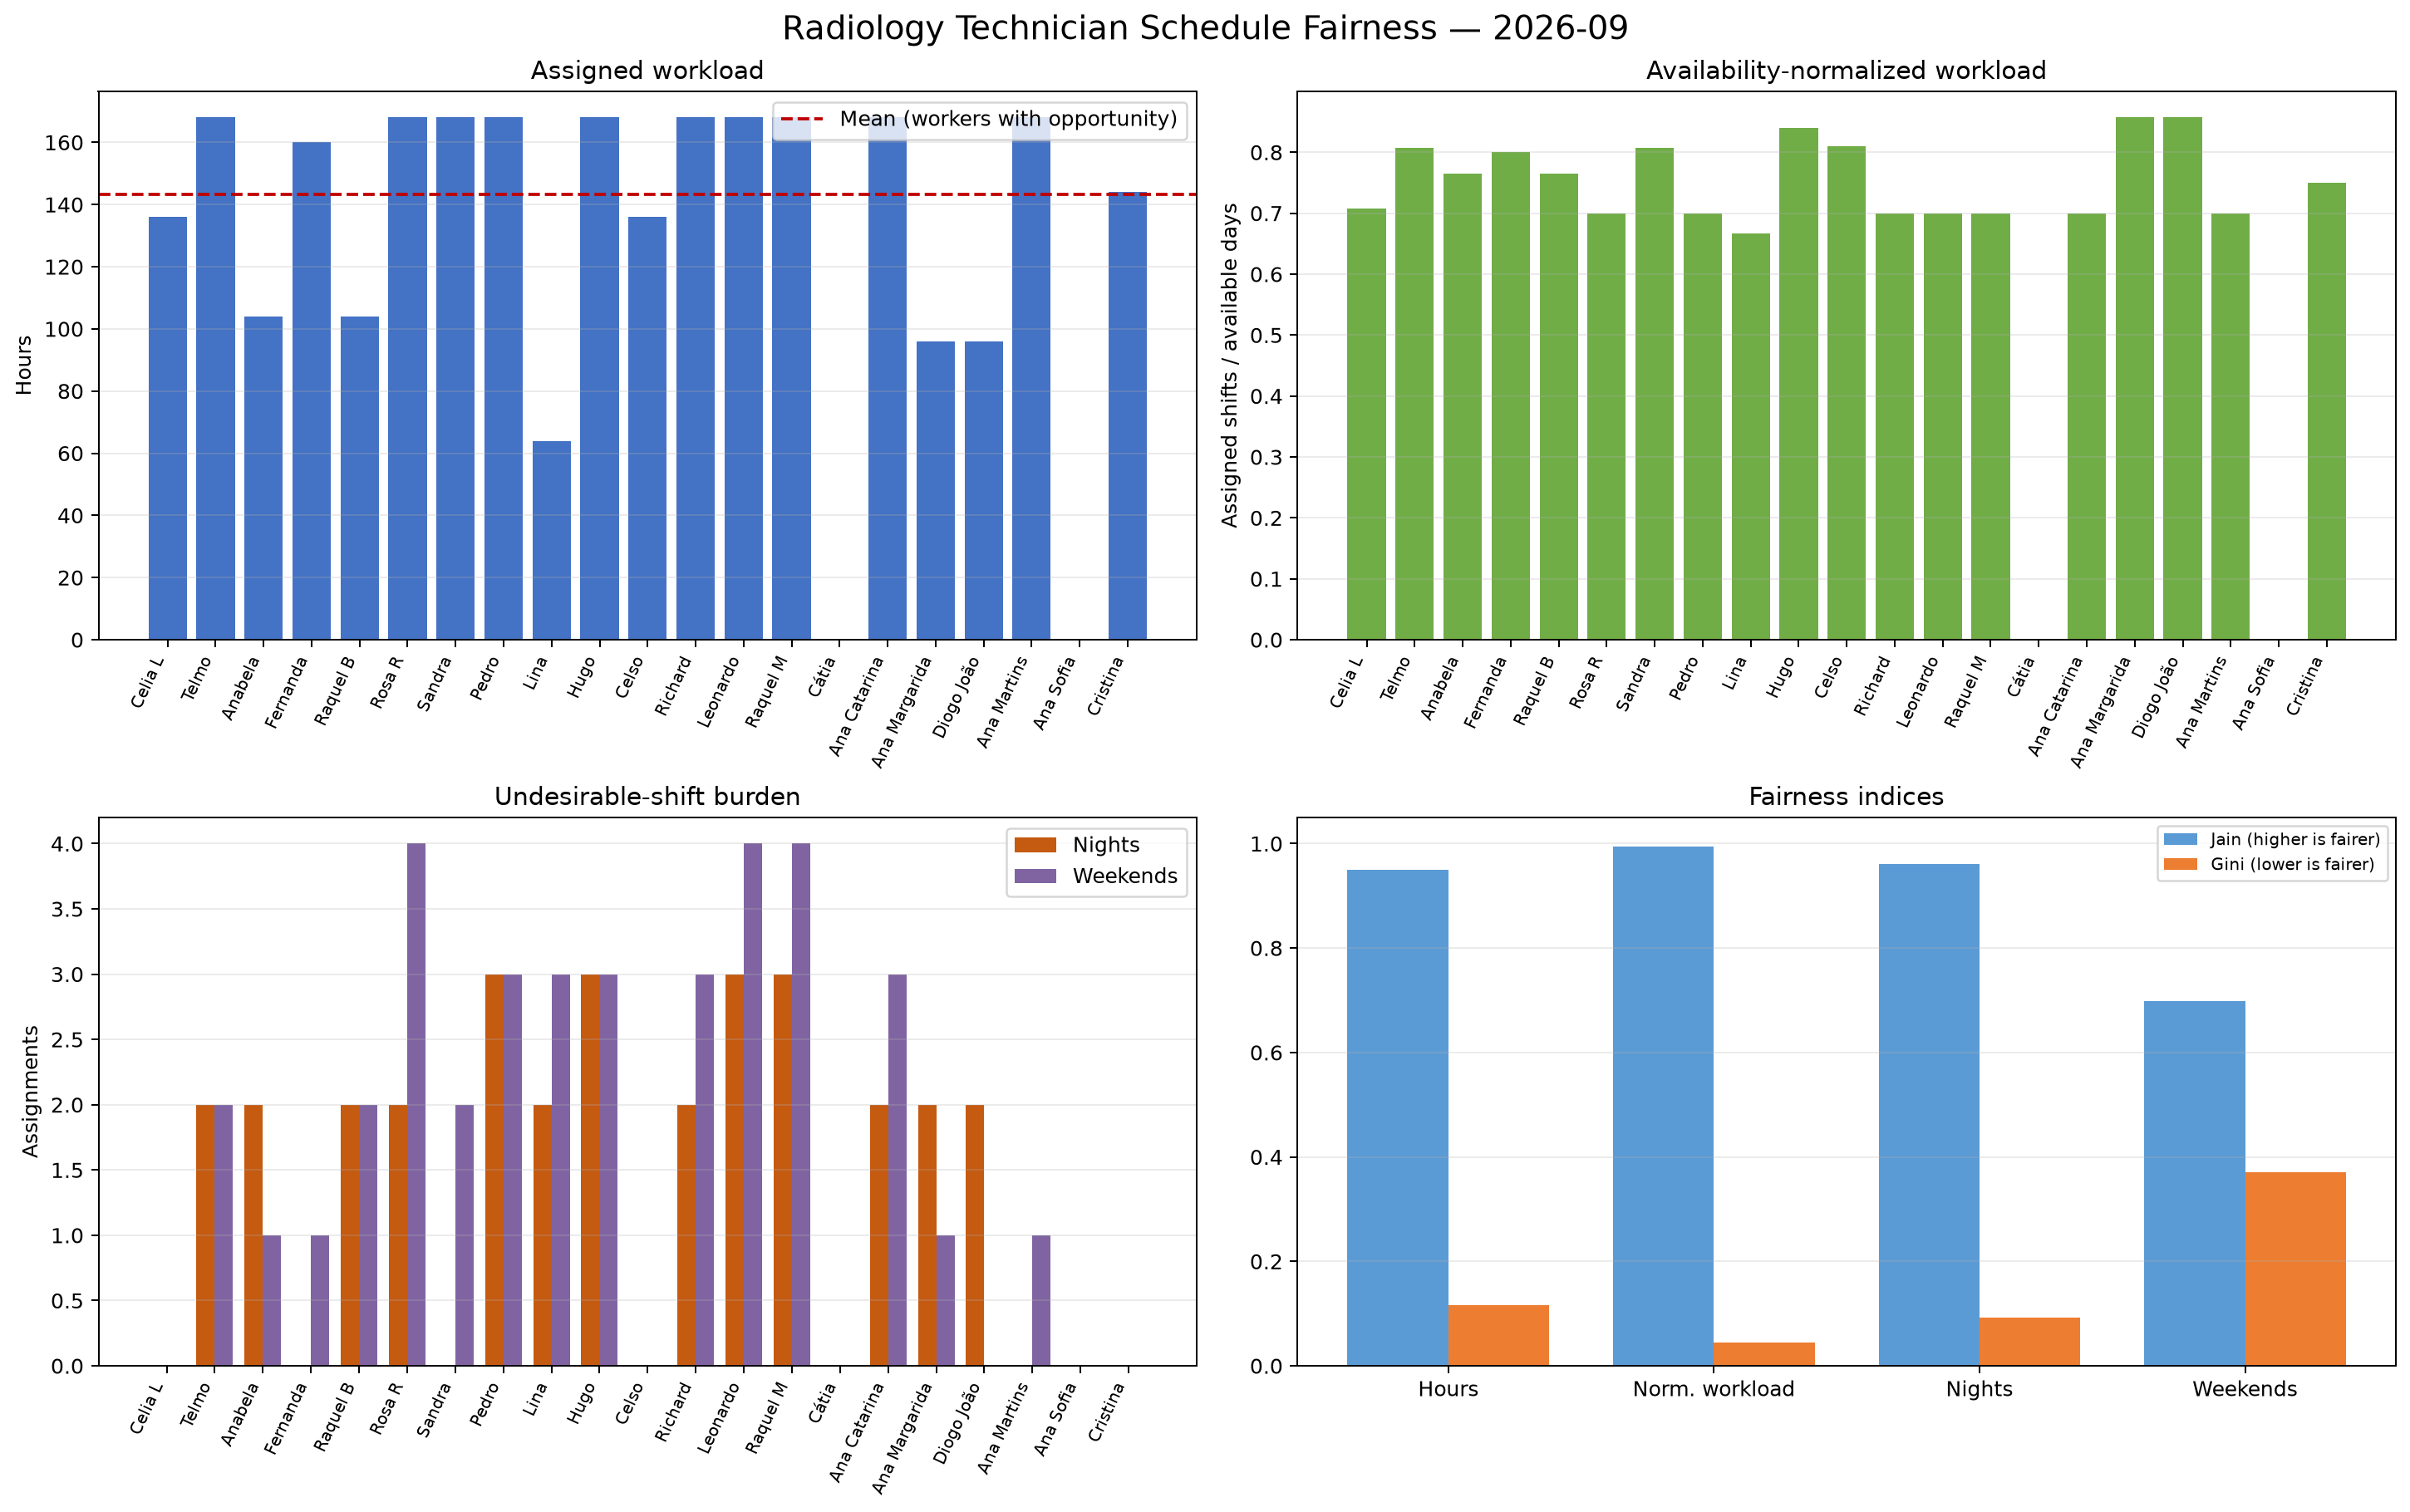
\includegraphics[width=0.94\textwidth]{fairness_dashboard.png}
  \caption{Fairness dashboard for the published Imaging roster. Top: raw assigned hours and workload normalised by available days. Bottom: each worker's night and weekend assignments and the corresponding Jain and Gini indices. Higher Jain and lower Gini values indicate a more even distribution; weekend burden is visibly less even than night burden.}
  \label{fig:fairness}
\end{figure}

\subsubsection{Sex-group results}

Table~\ref{tab:group-fairness} reports the post-hoc comparison of female and male Imaging workers in the published schedule. Raw night burden is greater for men: the mean worker-level rate is 11.23\% for men and 8.81\% for women. Raw weekend burden is slightly greater for women, at 17.27\% compared with 15.65\% for men.

Opportunity normalisation reverses the direction of both comparisons. The mean eligible-night rate is 11.12\% for women and 10.11\% for men, whereas the eligible-weekend rate is 47.57\% for women and 53.47\% for men. The combined raw burden score is very similar: 13.04\% for women and 13.44\% for men, as shown in Figure \ref{fig:group-fairness}. This reversal shows that the conclusion depends on whether equality is defined in relation to assignments received or opportunities available. These are descriptive differences in one small case study, not evidence of discrimination or a causal effect of sex.

\begin{table}[H]
\centering
\caption{Descriptive sex-group fairness results for the published schedule. Differences are female minus male; ratios are female divided by male.}
\label{tab:group-fairness}
\begin{tabularx}{\textwidth}{Xrrrr}
\toprule
Metric & Female & Male & Difference & Ratio \\
\midrule
Night shifts / assigned shifts & 0.0881 & 0.1123 & $-0.0242$ & 0.7845 \\
Weekend shifts / assigned shifts & 0.1727 & 0.1565 & 0.0162 & 1.1035 \\
Nights / eligible night opportunities & 0.1112 & 0.1011 & 0.0101 & 1.0999 \\
Weekend shifts / eligible weekend opportunities & 0.4757 & 0.5347 & $-0.0590$ & 0.8897 \\
Overall burden score & 0.1304 & 0.1344 & $-0.0040$ & 0.9702 \\
\bottomrule
\end{tabularx}
\end{table}

\begin{figure}[H]
  \centering
  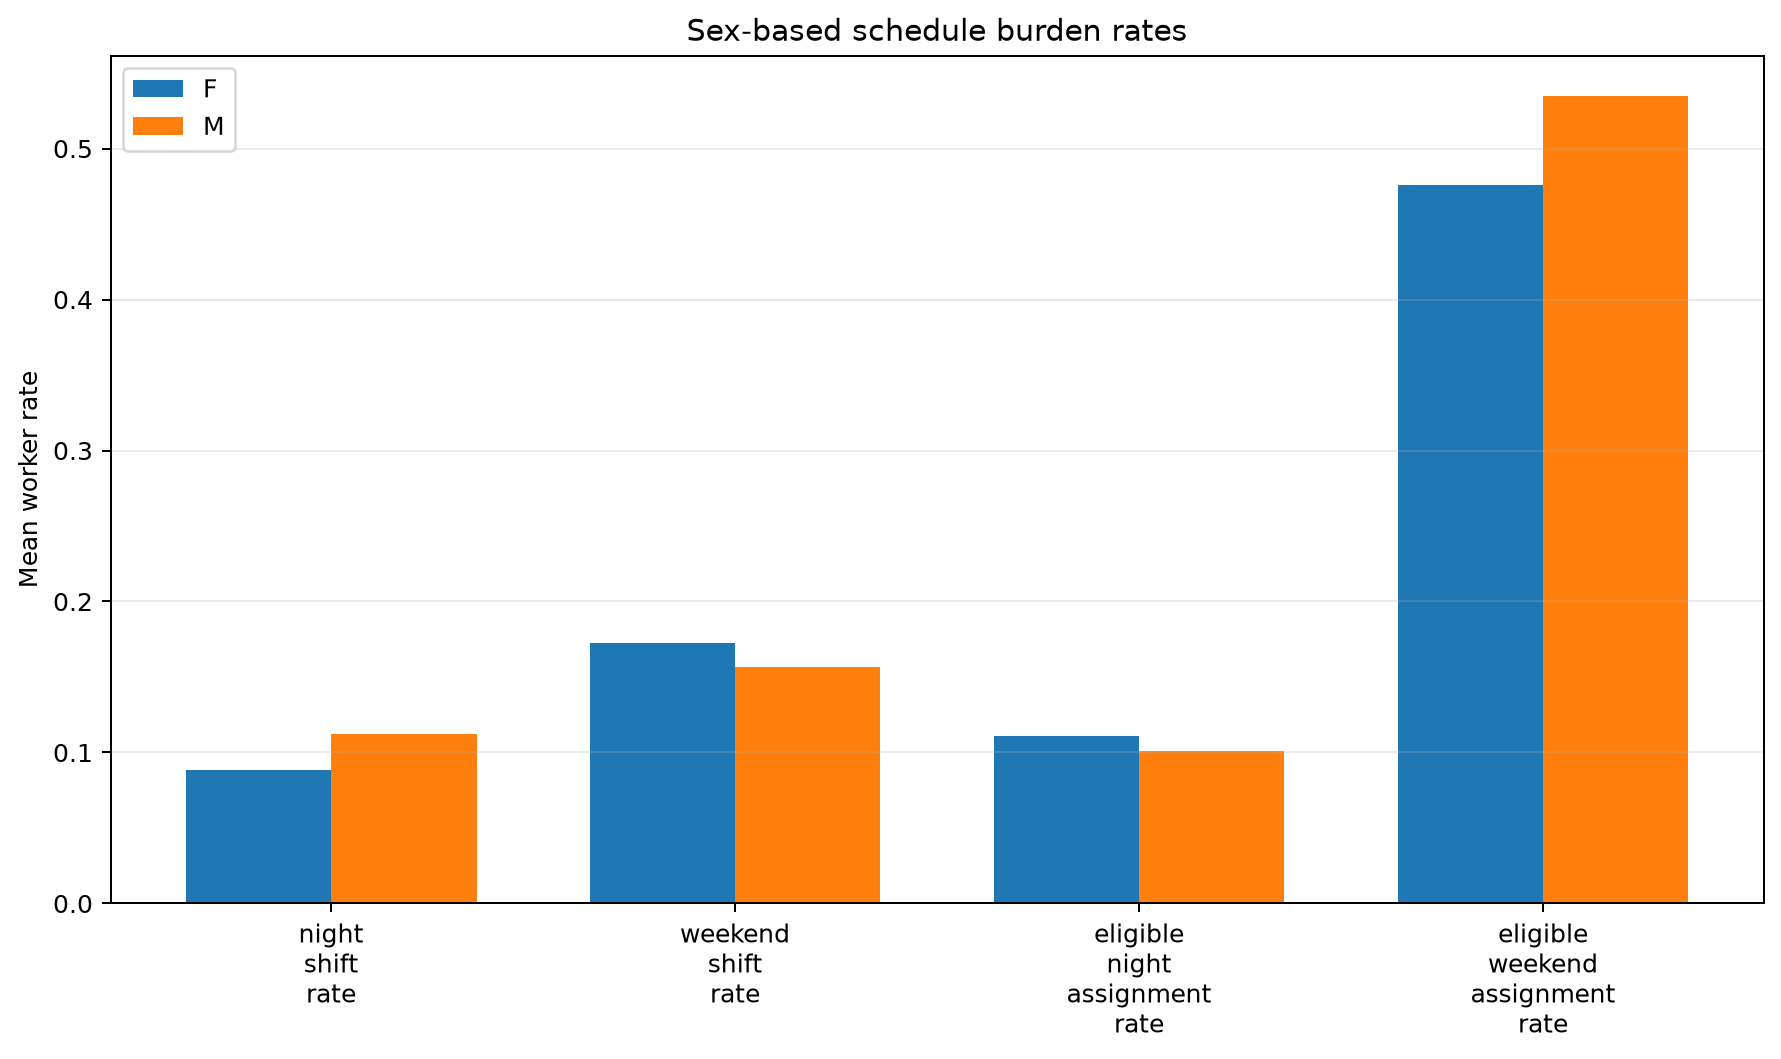
\includegraphics[width=0.75\textwidth]{../reports/fairness/sex_fairness_rates.png}
  \caption{Female and male shift-burden rates in the published schedule. Raw rates use assigned shifts as the denominator; eligible rates use static opportunities after accounting for absences, shift eligibility and Lina's linked Hemodynamics assignments.}
  \label{fig:group-fairness}
\end{figure}


\subsection{Trade-off experiment results}
\label{sec:tradeoff-results}

The four alternative profiles defined in the Trustworthy-AI analysis and the published schedule produce different distributions even though they use identical workers and hard constraints. Because their objective weights differ, their raw objective values are not directly comparable. Table~\ref{tab:profiles} therefore reports both Gini and Jain indices for availability-normalised workload, night burden and weekend burden, together with the common preference cost described above. The preference cost includes workload imbalance as well as workday imbalance, undesirable work/rest patterns, night preparation, holiday and weekend patterns, morning shortfall and overtime. It has no unit and lower values indicate fewer or smaller raw penalties. Figure~\ref{fig:tradeoffs} complements the table by visualising how these differences translate into alternative distributive outcomes. Panel (a) compares weekend fairness with aggregate preference cost, while panel (b) shows how the three Gini-based fairness measures vary across the five schedules.

All five schedules have highly even availability-normalised workload: Gini ranges only from 0.0426 to 0.0445 and Jain from 0.9936 to 0.9944. The weekend-focused profile produces by far the most even weekend allocation ($G=0.0859$, $J=0.9710$), while the published schedule has the least even weekend result ($G=0.3079$, $J=0.7562$). Conversely, the published schedule has the best normalised night distribution ($G=0.1631$, $J=0.9221$). This redistribution of fairness across dimensions is particularly visible in Figure~\ref{fig:tradeoffs}(b): improving equality in one burden category does not necessarily improve equality in the others. Figure~\ref{fig:tradeoffs}(a) further shows that greater weekend equality is not associated with a simple monotonic increase in aggregate preference cost; rather, the profiles occupy different positions according to the priorities encoded in their objective weights. Preference-cost values range narrowly from 11,376 to 11,516 and are dominated by the workload-imbalance component common to this evaluation. The profile names describe which penalties receive weight during optimisation, whereas the table measures the schedules after solving. The operational baseline is proven optimal. The remaining relative optimality gaps are approximately 0.0019\% for the workload-focused profile, 0.0245\% for the weekend-focused profile, 0.0607\% for the preference-focused profile, and 0.0090\% for the published schedule. These small gaps quantify the distance between each returned objective and its solver bound. The alternative runs reached their 60-second limits and the published run reached its 600-second limit, so the comparison describes the schedules found rather than definitive optima for every weighting policy.

\begin{table}[H]
\centering
\caption{Comparison of objective profiles. ``Gap'' is the relative difference between the returned objective and the solver's best bound; 0\% indicates a solver-certified optimum.}
\label{tab:profiles}
\small
\resizebox{\textwidth}{!}{%
\begin{tabular}{llrrrrrrrr}
\toprule
Profile & Status & Gap & Work $G$ & Work $J$ & Night $G$ & Night $J$ & Weekend $G$ & Weekend $J$ & Preference cost \\
\midrule
Operational baseline & Optimal & 0\% & 0.0426 & 0.9944 & 0.2136 & 0.8404 & 0.1512 & 0.9202 & 11,516 \\
Workload-focused & Feasible & 0.0019\% & 0.0445 & 0.9936 & 0.2206 & 0.8352 & 0.2848 & 0.7862 & 11,397 \\
Weekend-focused & Feasible & 0.0245\% & 0.0437 & 0.9938 & 0.2136 & 0.8404 & 0.0859 & 0.9710 & 11,391 \\
Preference-focused & Feasible & 0.0607\% & 0.0431 & 0.9939 & 0.2178 & 0.8382 & 0.1767 & 0.9071 & 11,376 \\
Published schedule & Feasible & 0.0090\% & 0.0445 & 0.9936 & 0.1631 & 0.9221 & 0.3079 & 0.7562 & 11,387 \\
\bottomrule
\end{tabular}
}
\end{table}

\begin{figure}[H]
  \centering
  \begin{subfigure}{0.49\textwidth}
    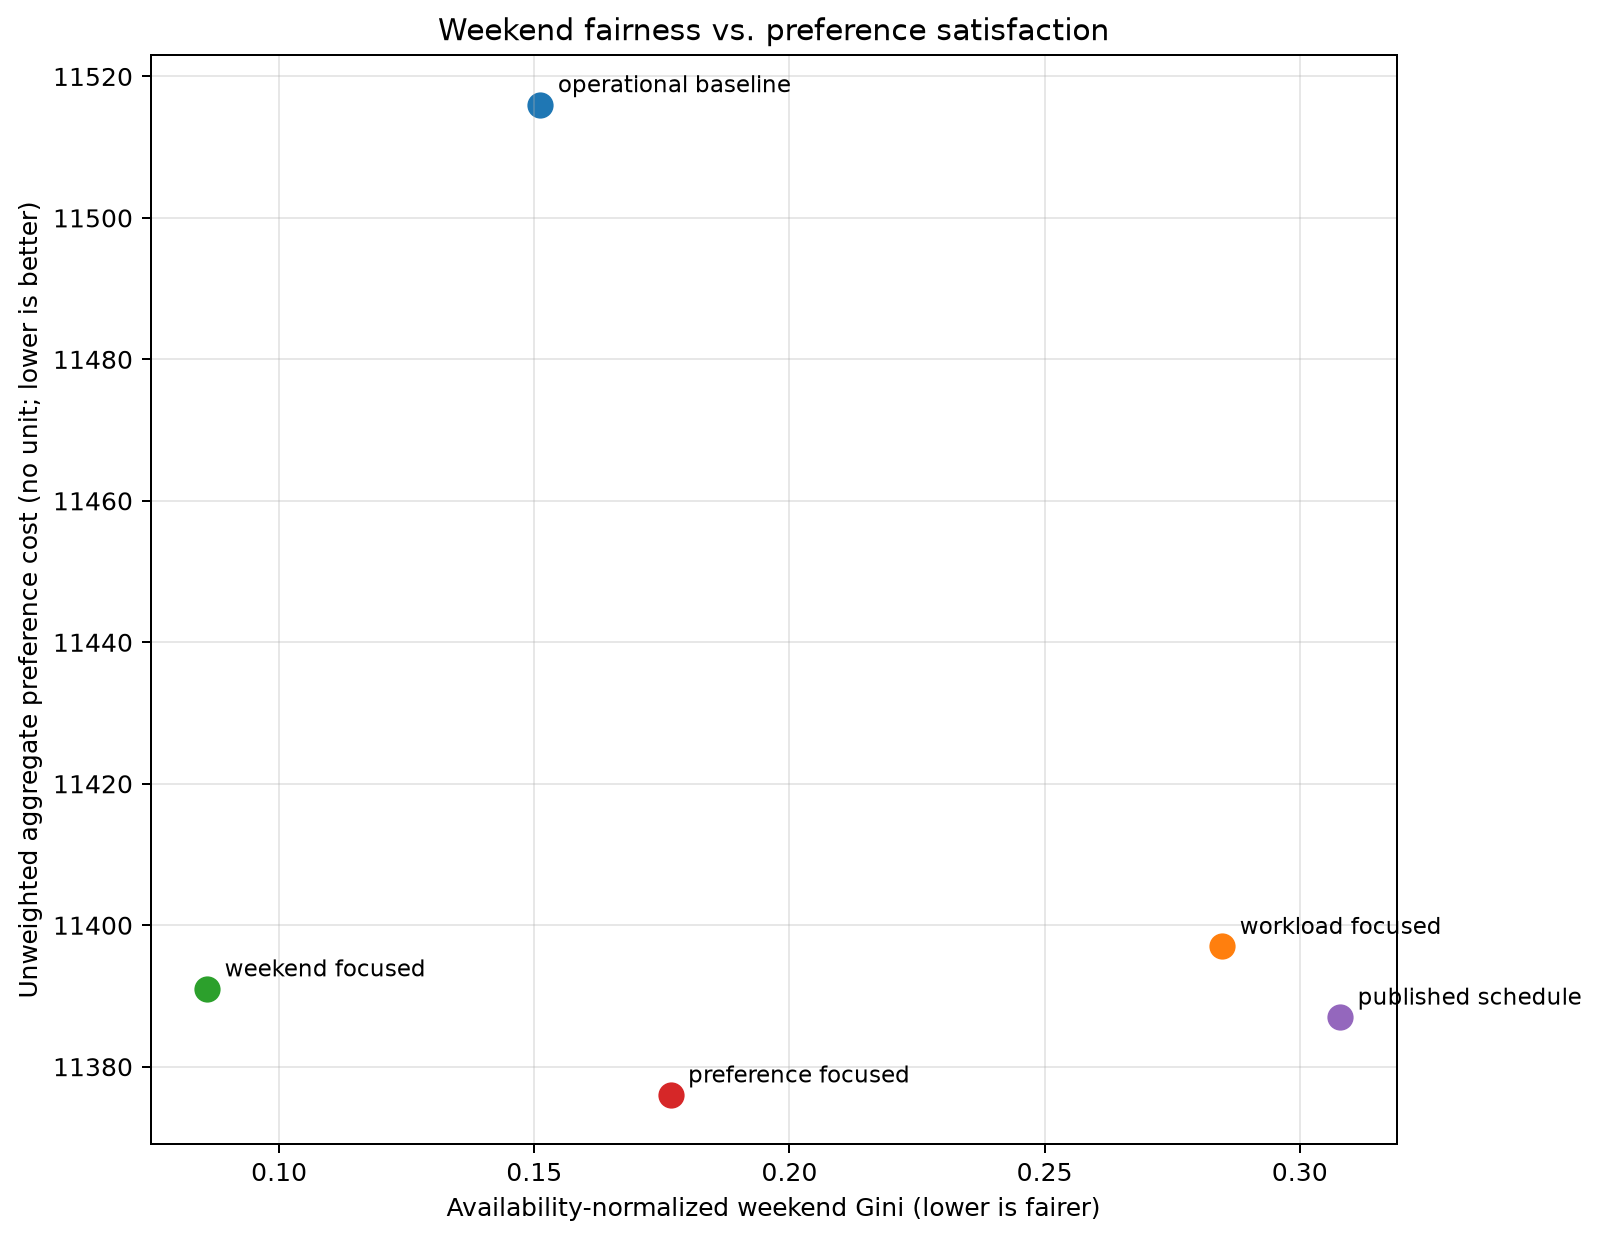
\includegraphics[width=\textwidth]{tradeoff_plot.png}
    \caption{Fairness--preference trade-off.}
  \end{subfigure}
  \hfill
  \begin{subfigure}{0.49\textwidth}
    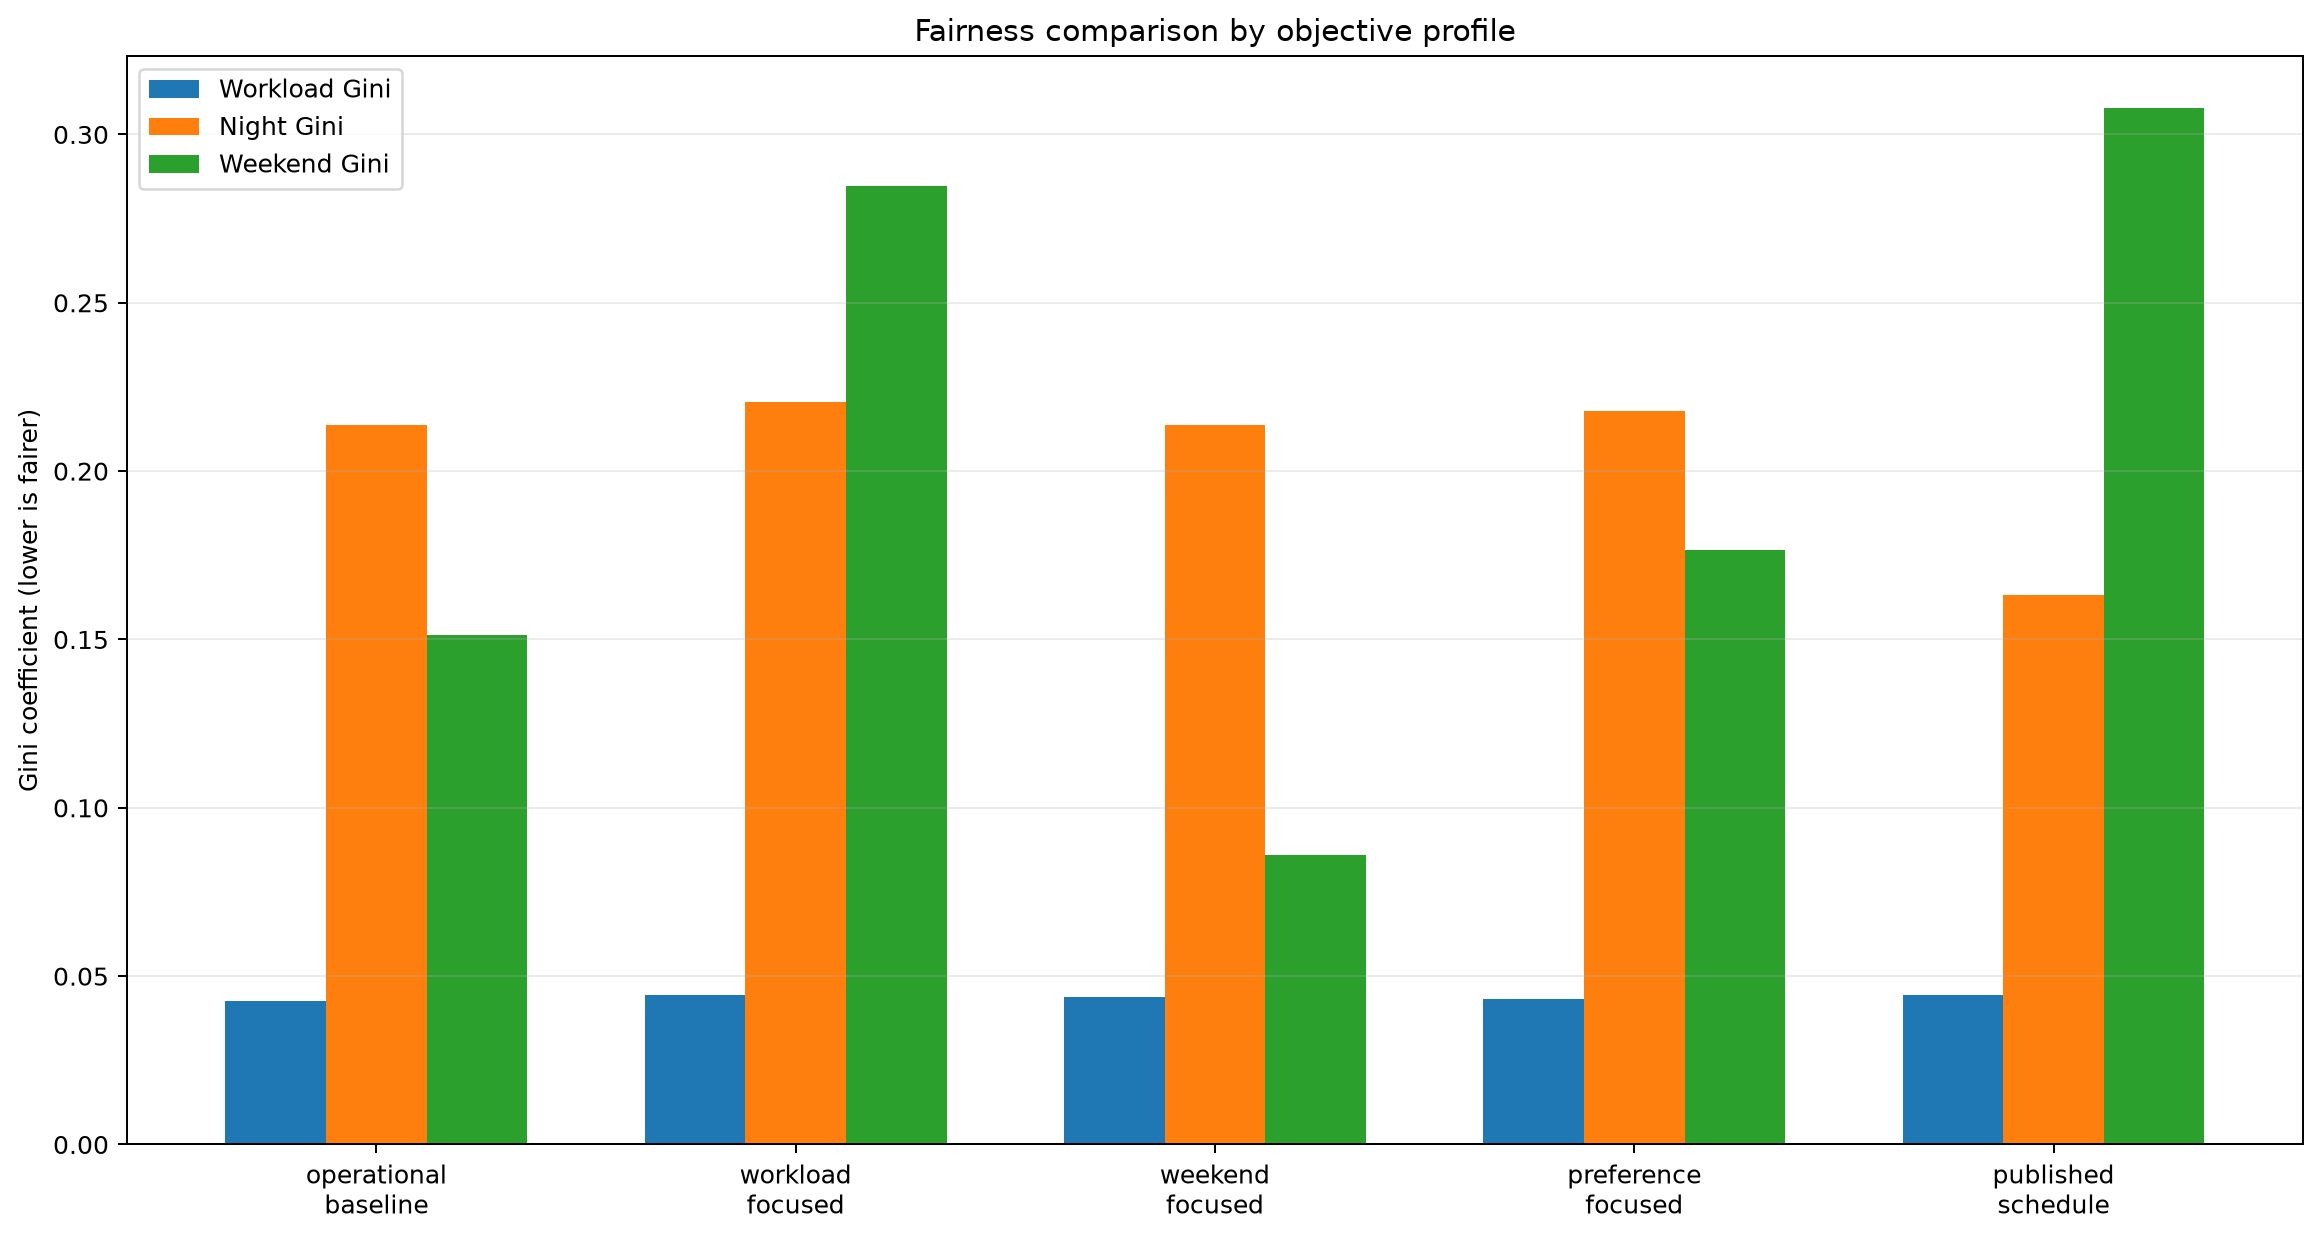
\includegraphics[width=\textwidth]{fairness_comparison.png}
    \caption{Fairness indices across profiles.}
  \end{subfigure}
  \caption{Objective weights select different distributive outcomes; no profile dominates on every measure.}
  \label{fig:tradeoffs}
\end{figure}

\subsection{Robustness results}

We studied six disruptions to the published schedule. All six scenarios produced solver-certified optimal repairs in less than one second. As summarised in Table \ref{tab:robustness}, the repairs changed two to 12 assignment rows, corresponding to one to six replacement-equivalent changes, and affected one to five workers.
Figure~\ref{fig:robustness} highlights the resulting disruption: most scenarios require only limited changes, while simultaneous absences produce the largest repair, with six replacements affecting five workers. Fairness effects remain small overall, with availability-normalised workload Gini changes between $-0.0008$ and $0$, night Gini changes between $-0.0161$ and $+0.0431$, and weekend Gini changes between $-0.0278$ and $+0.0026$.

These results show that feasible repairs exist for the tested perturbations, but also that a local disruption can require changes for several workers when the system is operating close to its capacity floor.

\begin{table}[H]
\centering
\caption{Robustness scenarios and schedule disruption. $\Delta G_W$, $\Delta G_NB$ and $\Delta G_WB$ denote changes in availability-normalised workload, night-burden and weekend-burden Gini coefficients, respectively.}
\label{tab:robustness}
\small
\begin{tabularx}{\textwidth}{Xrrrrrr}
\toprule
Scenario & Edits & Replacements & Workers & $\Delta G_W$ & $\Delta G_NB$ & $\Delta G_WB$ \\
\midrule
Single-day absence & 4 & 2 & 2 & $-0.0003$ & $-0.0013$ & $+0.0026$ \\
Night-worker absence & 4 & 2 & 2 & $-0.0003$ & $-0.0013$ & 0.0000 \\
Three-day absence & 6 & 3 & 2 & $-0.0005$ & $-0.0041$ & $+0.0026$ \\
Morning-demand increase & 2 & 1 & 1 & 0.0000 & 0.0000 & $-0.0278$ \\
Night-demand increase & 3 & 2 & 2 & $-0.0004$ & $+0.0431$ & $+0.0026$ \\
Simultaneous absences & 12 & 6 & 5 & $-0.0008$ & $-0.0161$ & $-0.0149$ \\
\bottomrule
\end{tabularx}
\end{table}

\begin{figure}[H]
  \centering
  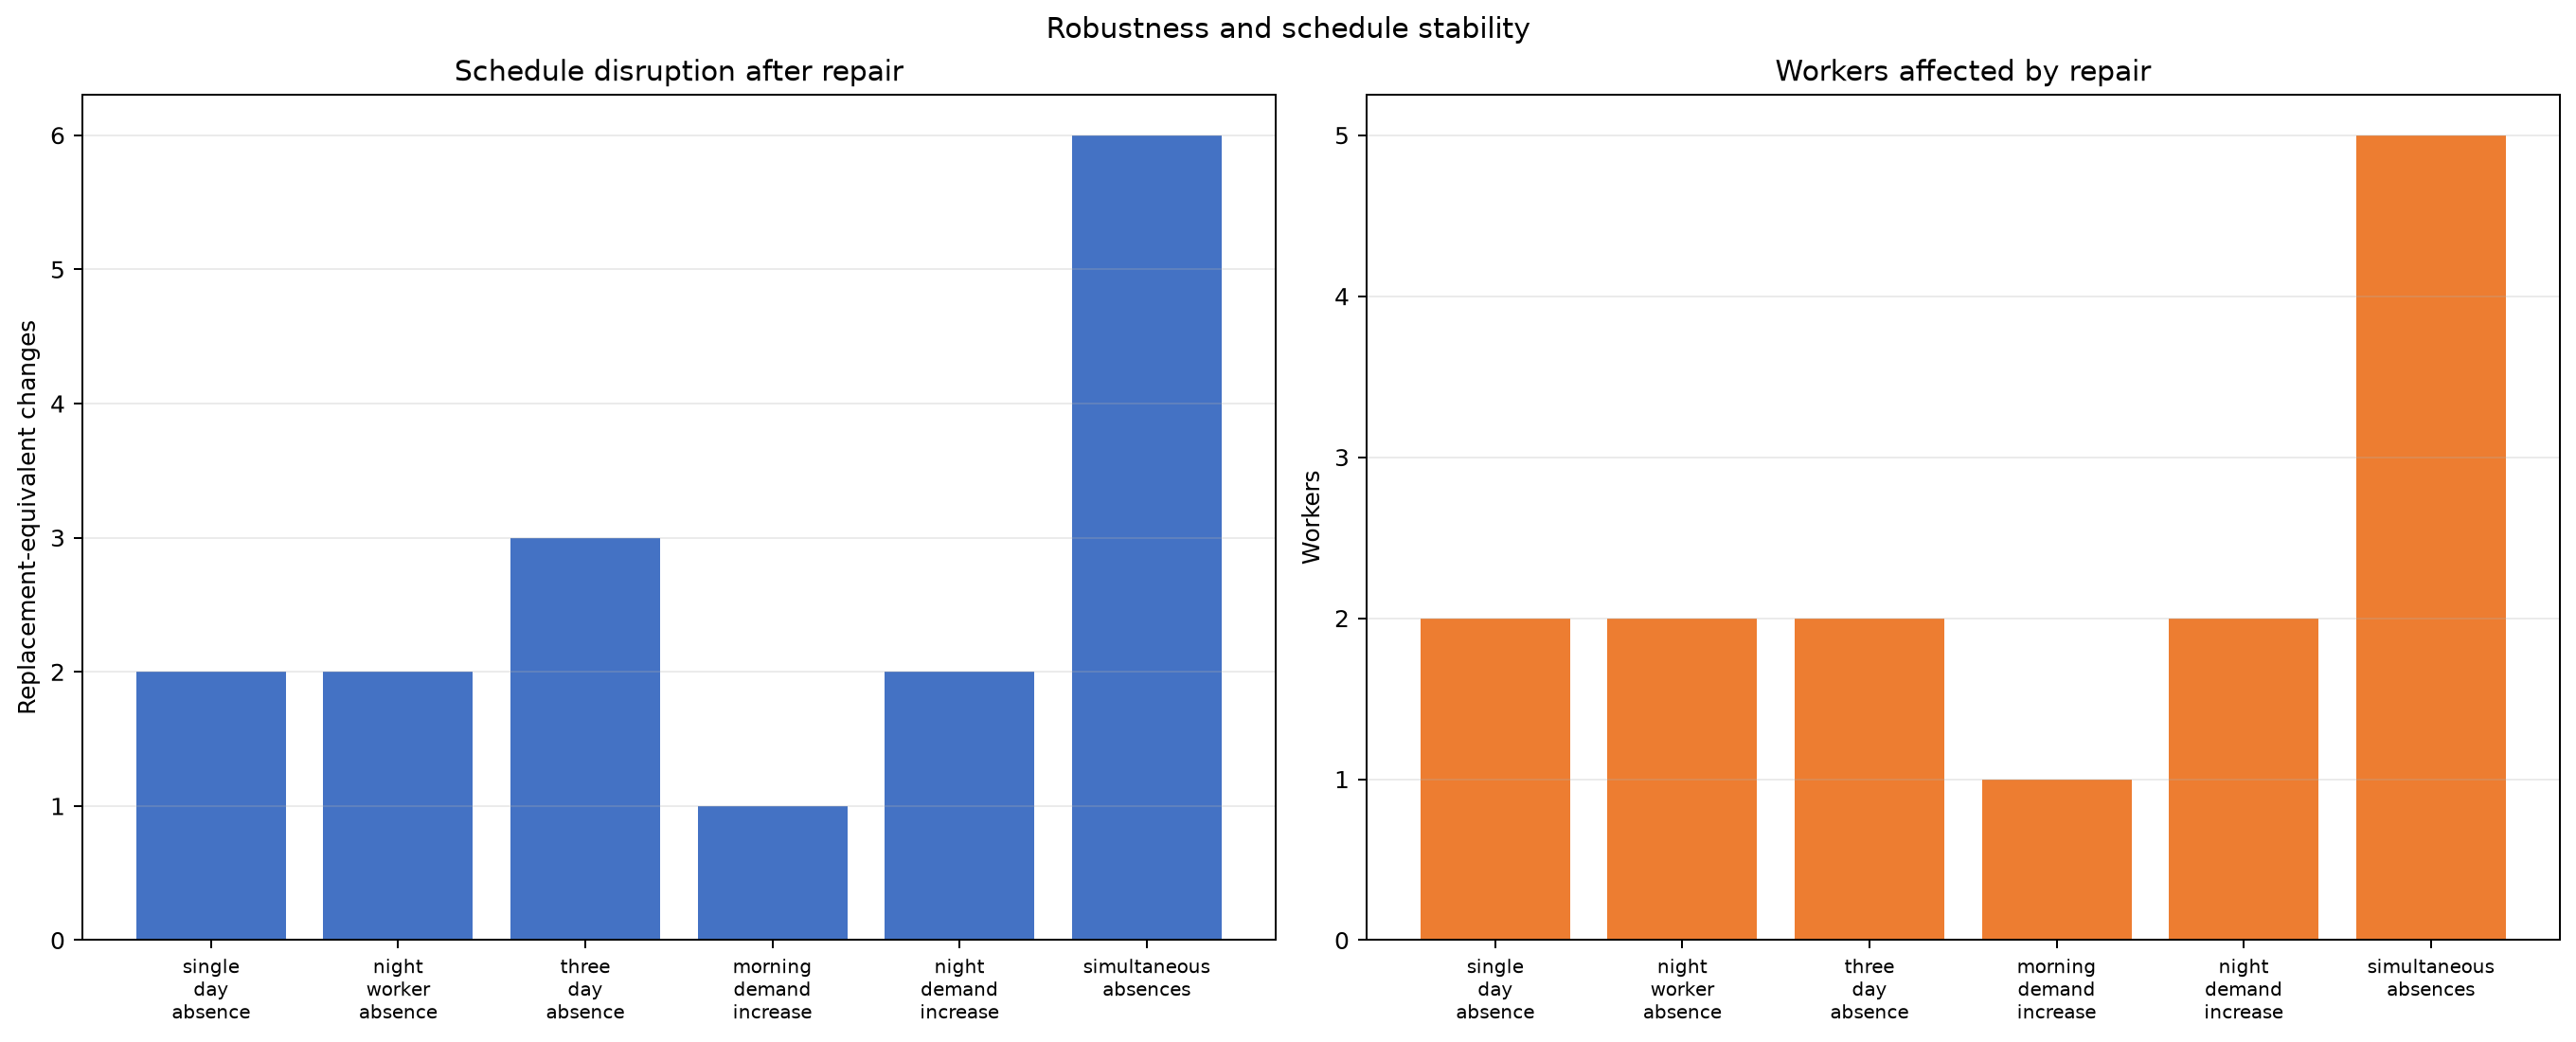
\includegraphics[width=0.92\textwidth]{stability_chart.png}
  \caption{Schedule disruption under controlled perturbations. Left: replacement-equivalent assignment changes required by each repair. Right: number of workers whose assignments are affected.}
  \label{fig:robustness}
\end{figure}

\subsection{Explanation examples}

The system checked 340 scheduled Imaging assignments and generated 2,158 ``why not this worker?'' records. Of those alternatives, 2,015 (93.37\%) had at least one direct blocking reason. The other 143 had no single visible blocker, so the report states only that another assignment was selected by the overall objective.

Figure~\ref{fig:objective-contributions} decomposes the objective value of the published schedule into its weighted components, accounting for the score at the returned solution. The coefficients were specified before solving. The two key-day morning shortfalls (one missing worker on Wednesday, 9 September and one on Friday, 11 September) contribute $20{,}000{,}000$ points, or 86.1\% of the final score. Cumulative workday balance contributes 9.0\% and workload deviation 4.7\%; all remaining components together contribute less than 0.2\%. These percentages show how the configured weights and the violations combine to produce the returned objective value; they are not weights learned from data. The separate staffing counterfactual proves that the one-worker gap on 11 September cannot be removed under the encoded hard constraints, so this specific heavily penalised shortfall is necessary in this month. The 9 September gap can be moved by rescheduling, although eliminating it locally has consequences elsewhere.

\begin{figure}[H]
  \centering
  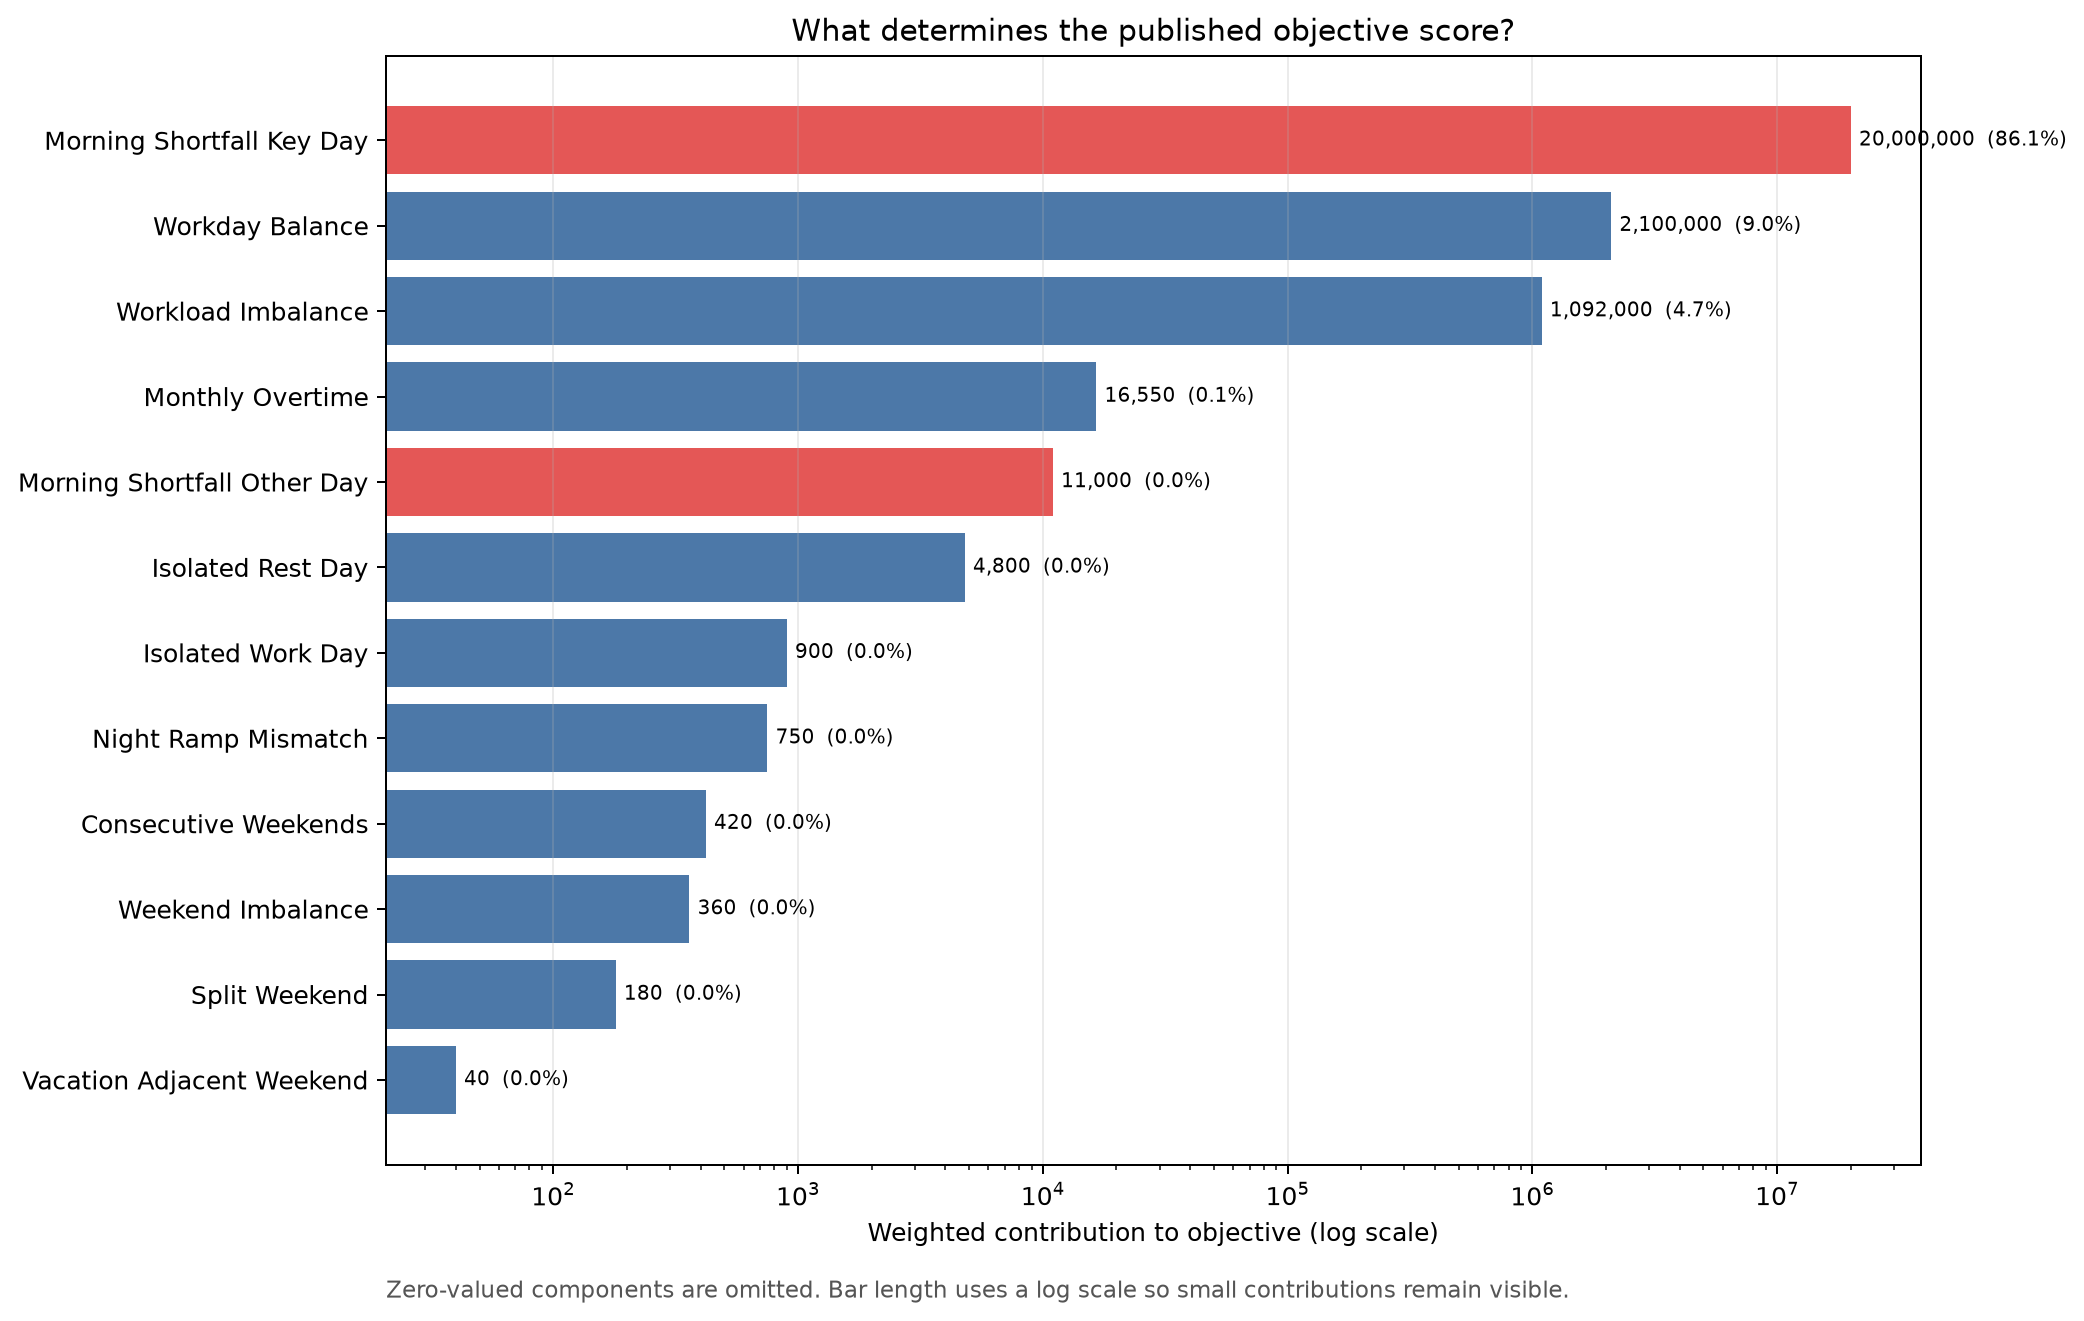
\includegraphics[width=0.9\textwidth]{../reports/report_visualizations/02_objective_contributions.png}
  \caption{Weighted contributions to the published schedule's objective value. The horizontal axis is logarithmic so that small non-zero components remain visible. Zero-valued components are omitted. The percentages decompose the returned score; they are not learned parameters or causal importance estimates.}
  \label{fig:objective-contributions}
\end{figure}

For a concrete assignment counterfactual, Leonardo's night shift on 10 September was forbidden. The solver found an optimal repair, showing that Leonardo was not indispensable on that night. Figure~\ref{fig:counterfactual-changes} shows the resulting reassignment: Leonardo’s night shift on 10 September and Richard’s morning shift on 11 September are removed, while Richard takes the night shift and Leonardo the following morning, requiring four assignment edits affecting two workers. Both schedules were evaluated with the published objective weights. The score increased from $23{,}227{,}000$ to $23{,}228{,}550$, a deterioration of 1,550 points. Of this increase, 800 points come from four additional isolated-rest penalties, 600 from two additional isolated-work penalties and 150 from one additional night-preparation mismatch. The reported fairness indices do not change. The explanation is therefore not ``Leonardo had to work.'' It is ``another valid choice existed, but it produced less desirable work/rest and night-preparation patterns according to the objective.''

\begin{figure}[H]
  \centering
  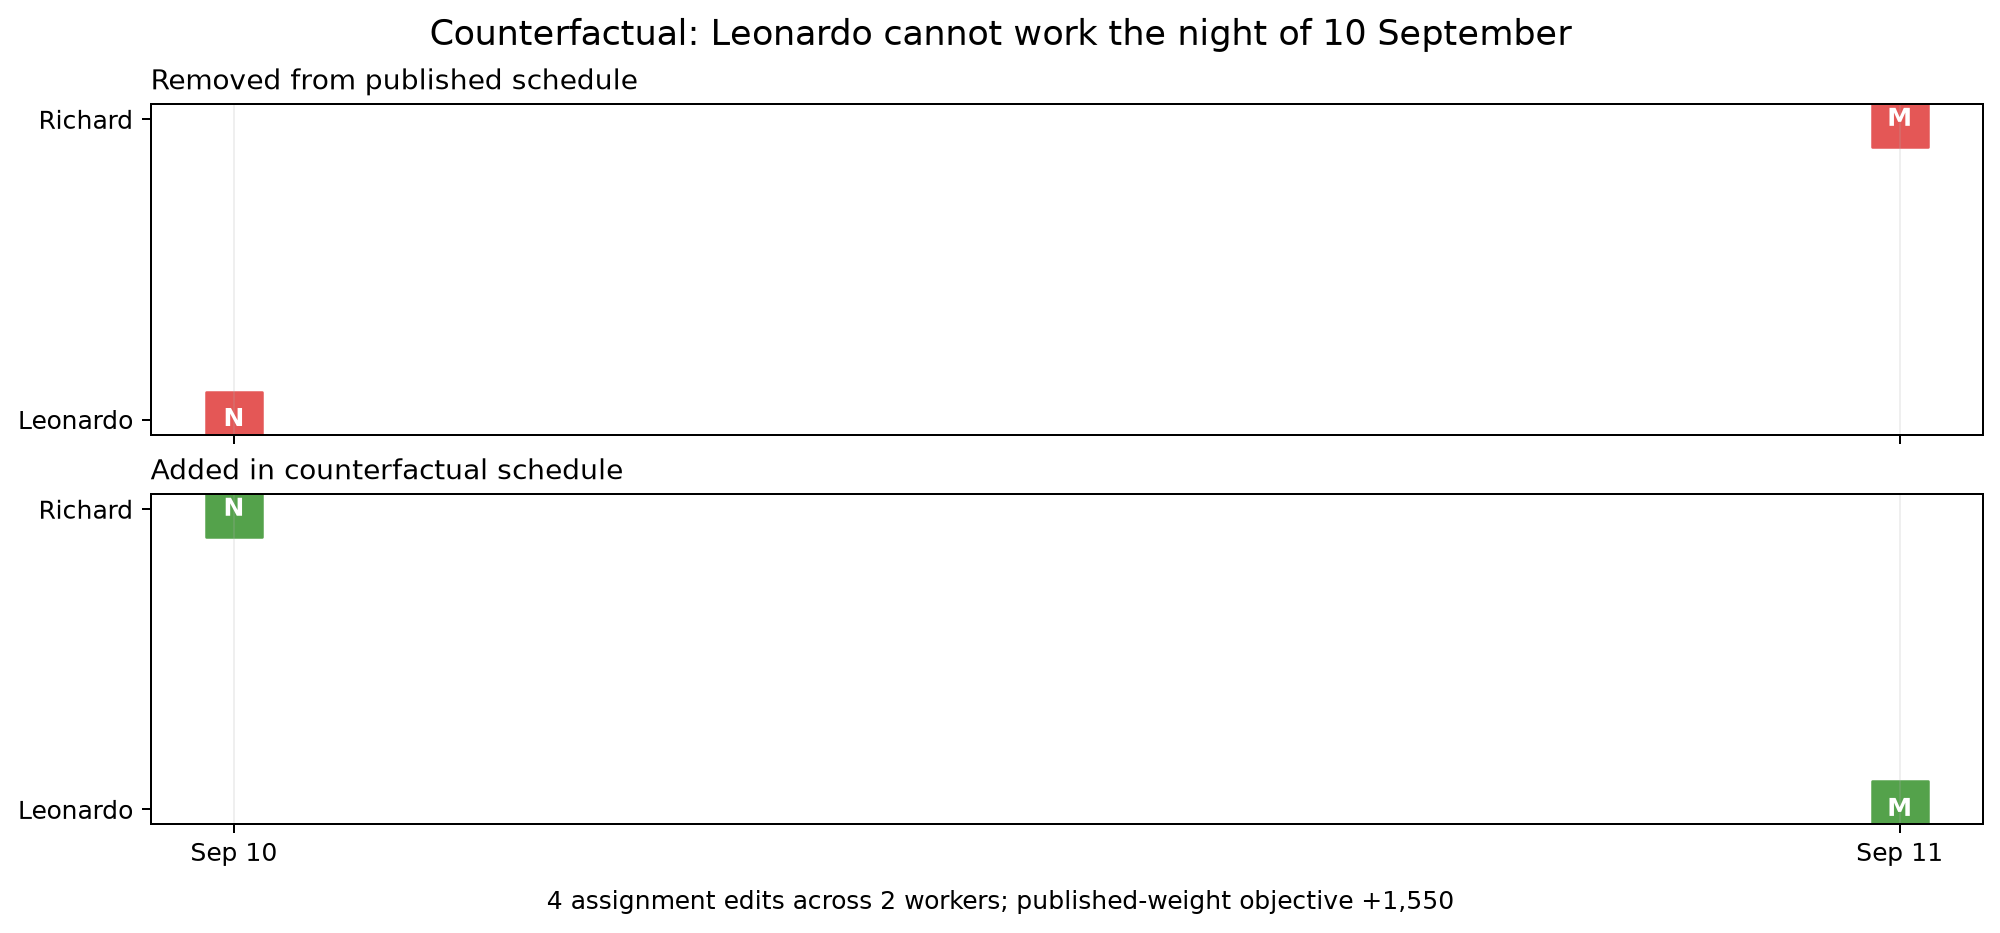
\includegraphics[width=0.9\textwidth]{../reports/report_visualizations/05_counterfactual_changes.png}
  \caption{Exact assignment changes after forbidding Leonardo's night shift on 10 September. Leonardo and Richard exchange the night and following-morning assignments, producing four edits. The alternative remains feasible but scores 1,550 points worse under the published weights.}
  \label{fig:counterfactual-changes}
\end{figure}

The shortfall counterfactuals answer a different and operationally more important question. Eight of the nine affected mornings can individually reach the preferred target of 10 through rescheduling, but 11 September cannot. Moreover, all weekday mornings cannot reach 10 simultaneously: the proven minimum total gap is 17 worker-slots, compared with 24 in the published schedule. The schedule returned by this gap-only diagnostic uses 384 overtime hours, compared with 331 in the published schedule. These results make the actual compromise visible: most individual gaps can be relocated, but some month-wide shortage and the 11 September gap are unavoidable under the encoded constraints.

Figure~\ref{fig:staffing-overtime-outcomes} places this result beside the schedules generated for the objective-profile experiment. The points illustrate outcomes that were actually found: lower overtime is associated with larger preferred-target gaps, while the proven minimum-gap schedule requires substantially more overtime.

\begin{figure}[H]
  \centering
  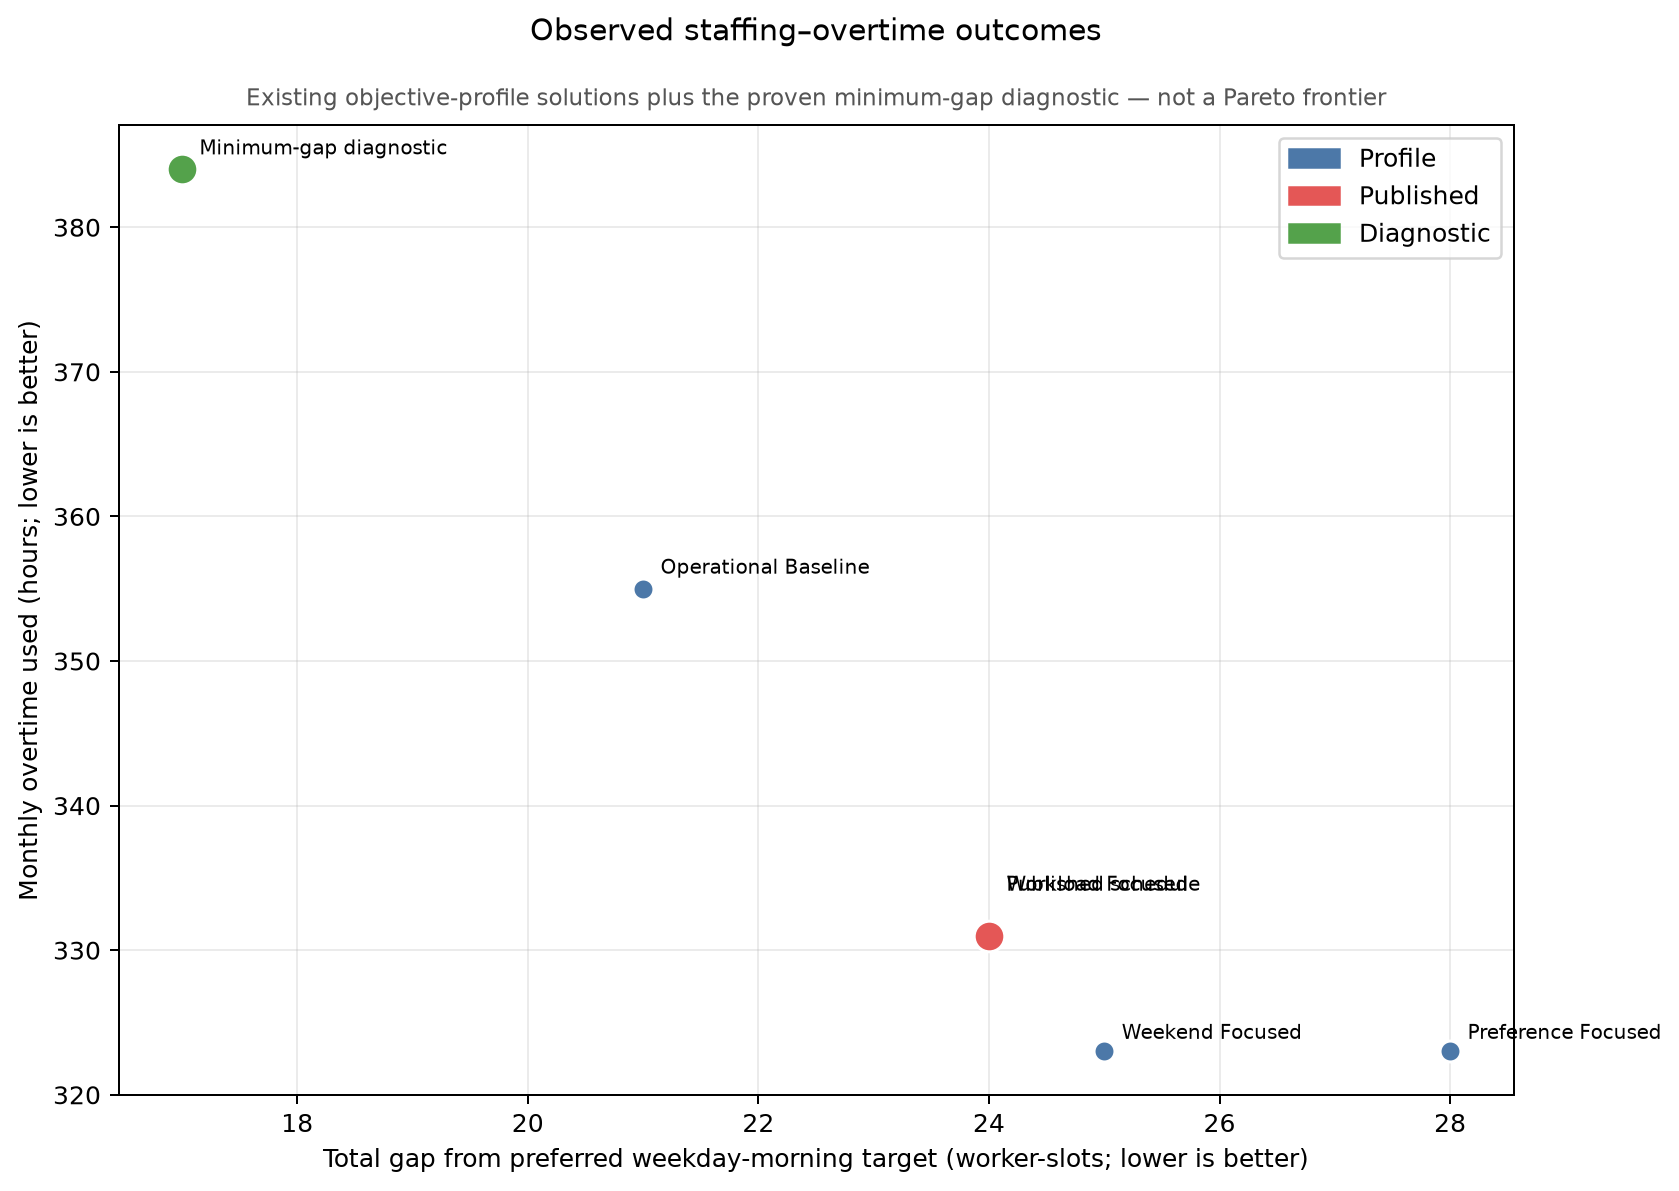
\includegraphics[width=0.8\textwidth]{../reports/report_visualizations/01_staffing_overtime_tradeoff.png}
  \caption{Observed weekday-morning shortfall and overtime outcomes. The published schedule has a gap of 24 worker-slots and 331 overtime hours. A gap-only optimisation proves a minimum gap of 17; its returned schedule uses 384 overtime hours. Profile points represent comparison schedules generated with different weights.}
  \label{fig:staffing-overtime-outcomes}
\end{figure}

These explanations support contestability. A scheduler or worker can challenge an input fact, a rule, an objective weight or the practical acceptability of the staffing/overtime trade-off.

\section{Ethical Discussion}

\subsection{What ``fair'' means in this system}

The project interprets fairness as a family of inspectable distributions. Equality of raw workload rewards equal totals; equity relative to availability adjusts for opportunity; burden sharing focuses on nights and weekends; temporal fairness carries workday and holiday history across months. These principles can conflict. Equal hours may overload a worker with limited availability, while equal opportunity-normalised ratios may create unequal pay or totals. The appropriate balance requires institutional and worker participation, not only optimisation, because abstract fairness metrics cannot capture the full organisational context \cite{selbst}.

Overtime makes this distinction even more important. When staffing demand cannot be met within ordinary contractual hours, perfect equality may be impossible: one or more workers must accept additional hours and operational restrictions may make only a subset eligible. The relevant fairness question is then not whether every worker receives an identical total, but whether the unequal burden is necessary, proportionate, transparently calculated and fairly rotated over time. The model represents overtime explicitly, penalises its use, bounds the amount assigned to an overtime worker and reports the resulting allocation. This is preferable to leaving the choice implicit in a manually assembled roster.

Using a solver can also support procedural consistency. Given the same model, data and solver conditions, it applies the encoded criteria without introducing undocumented case-by-case judgements. This can reduce opportunities for inconsistent treatment and make decisions easier to audit. Nevertheless, consistency of the computation is not neutrality of the whole system: input data may be incomplete, worker-specific constraints may be represented incorrectly, and weights can privilege some interests over others. Human oversight is therefore needed to define legitimate rules, inspect unequal outcomes and correct the model.

The night-fairness band is a relatively strong distributive commitment because it constrains eligible workers to floor/ceiling shares. Other fairness goals are weighted and can be traded against pattern preferences or staffing. The reports make that distinction visible.

\subsection{Human oversight and contestability}

The intended workflow is human-in-the-loop. Before publishing a monthly timetable, a scheduler should verify inputs, coverage, overtime, compensatory rest and unusual worker-specific burdens. The service coordinator analyses the resulting schedule and may adjust constraints or generate a revised schedule.

\subsection{Privacy and data governance}

The use of employee data was authorised for this academic project, and all employee names used in the report were changed to protect individual identities. However, for real-life deployment, since the schedule contains personal and potentially sensitive employment information, access should be restricted to authorised users and generated reports should be stored and transmitted securely. Retention periods should also be defined, especially for sickness, vacation and historical burden data \cite{gdpr}.

\subsection{Failure modes}

Important failure modes include incomplete absence data, mistaken shift eligibility, outdated contractual hours, incorrect carry-over state, overconfident interpretation of a feasible status and weights that silently privilege one group or pattern. A second class of failures arises from model omission: skill mix, ward-specific competence and qualitative team considerations may not be fully represented. Finally, an explanation may be technically true yet misleading if it describes legality without mentioning a service-wide capacity shortfall. The reporting design mitigates, but cannot eliminate, these risks.

\section{Limitations}

The evaluation concerns one main month and a bounded set of synthetic disruptions. It does not constitute a prospective clinical deployment study. There is no comparison against historical manual schedules or worker satisfaction data, so claims about improved fairness or administrative time cannot yet be made. The objective weights have not been elicited through a formal multi-stakeholder process. The sex-group audit is descriptive, covers only 14 female and seven male workers, and includes no significance test or causal analysis. Its results are sensitive to the population, denominator and static opportunity definition. No other protected attributes were available, so intersectional comparisons and disparities involving age, disability or other characteristics could not be assessed.

The weekday-morning formulation now prevents coverage below six, while retaining 10 as the preferred target. A production interface should display both hard-floor compliance and distance from the operational target. It should also require explicit approval of the substantial overtime needed to maintain the floor.

A further limitation is that hospital scheduling requirements are not always easy to express as fixed numerical constraints. The appropriate staffing level may depend on contextual factors that are difficult to anticipate or quantify. For example, fewer technicians may be sufficient on a day with an unusually low number of scheduled examinations, while a larger team may be necessary when the assigned workers are less experienced or when the expected procedures are particularly demanding. Other relevant considerations may include the combination of competencies within a team, equipment availability, anticipated emergencies and informal knowledge of how the department operates. Capturing all these nuances in advance would require richer and continually updated data and some factors may remain inherently difficult to formalise. Human review is therefore necessary to identify missing context, correct unsuitable assumptions and approve or revise the generated schedule before it is used operationally.

Counterfactual explanations may be computationally expensive and can vary with the solver time limit. A result for one date must not be interpreted independently of the month: eight affected dates could individually be raised to 10 workers, 11 September could not and the system-wide experiment proved that all dates could not reach 10 simultaneously. Local compliance checks also do not provide a complete causal explanation of a global optimisation result. Finally, the minimum-gap experiment deliberately ignores fairness, schedule patterns and overtime cost, and the returned schedule uses 384 overtime hours.

\section{Conclusions and Future Work}

The project demonstrates that radiology scheduling can be represented as an auditable optimisation problem without reducing Trustworthy AI to a single fairness score. The implementation generates reproducible schedules, exposes mandatory rules and weighted compromises, measures distributional outcomes, repairs bounded disruptions and tests explanations by solving explicit alternatives.

The September case study has four central scheduling findings. First, availability-adjusted workload is highly even ($G=0.0445$, $J=0.9936$), and eligible workers receive two or three nights ($G=0.0923$, $J=0.9615$ for night counts). Weekend work is markedly less even ($G=0.3079$, $J=0.7562$ after opportunity normalisation), identifying a concrete area for future improvement. Second, the mandatory floor of six weekday-morning workers can be maintained, but the published schedule uses 331 overtime hours and has a total gap of 24 worker-slots from the preferred target. Third, robustness experiments further show that all six bounded disruptions could be repaired optimally with at most 12 assignment edits affecting five workers. Fourth, the explanation experiments show that most gaps can be relocated but some shortage is unavoidable: eight of the nine dates can individually reach 10, 11 September cannot, and the proven minimum total gap is 17. The schedule returned by that gap-only diagnostic uses 384 overtime hours. The published result is therefore a month-wide compromise between preferred coverage, overtime, fairness and schedule stability.

The post-hoc sex-group audit adds another finding. Raw night burden is higher for men (11.23\% versus 8.81\%), while raw weekend burden is slightly higher for women (17.27\% versus 15.65\%). After opportunity normalisation, night burden is slightly higher for women (11.12\% versus 10.11\%) and weekend burden is higher for men (53.47\% versus 47.57\%). The combined burden scores are close (13.04\% for women and 13.44\% for men). These results are descriptive rather than evidence of discrimination.

Future work should validate every constraint and weight with schedulers and worker representatives, compare generated and historical rosters, add formal skill-mix requirements, distinguish critical from negotiable coverage in the user interface and evaluate worker-perceived fairness. Longer multi-month experiments should test carried fairness and holiday rotation. A deployment study should measure correction rates, planning time, stability, contestation outcomes and whether explanations improve appropriate trust rather than simple acceptance.

\section{Reproducibility}

The following commands reproduce the September case study from the repository root. They use the same random seed and time limits as the reported results. First create the Python environment:

\begin{small}
\begin{verbatim}
python3 -m venv .venv
.venv/bin/pip install -r requirements.txt
\end{verbatim}
\end{small}

Generate the linked Hemodynamics and Imaging schedules together:

\begin{small}
\begin{verbatim}
.venv/bin/python solver.py --year 2026 --month 9 \
  --config config/2026-09.json --department both \
  --rest rest_hours.json --contracts contract_hours.json \
  --workday-history workday_history.json \
  --holidays holiday_rotation.json \
  --output reports/2026-09/schedule.csv \
  --hemodinamica-output reports/2026-09/hemodinamica_schedule.csv \
  --prevention-output reports/2026-09/prevention.csv \
  --compensation-output reports/2026-09/compensatory_rest.csv \
  --time-limit 600 --hemodinamica-time-limit 120
\end{verbatim}
\end{small}

Create the individual fairness, staffing and timetable outputs:

\begin{small}
\begin{verbatim}
.venv/bin/python evaluate.py reports/2026-09/schedule.csv \
  --config config/2026-09.json \
  --hemodinamica-schedule reports/2026-09/hemodinamica_schedule.csv \
  --json reports/2026-09/fairness_report.json \
  --csv reports/2026-09/fairness_workers.csv \
  --chart reports/2026-09/fairness_dashboard.png \
  --attributes config/worker_attributes.json \
  --solver-report reports/2026-09/solver_report.json

.venv/bin/python staffing_report.py reports/2026-09/schedule.csv \
  --report reports/2026-09/solver_report.json \
  --holidays holiday_rotation.json --output-dir reports/2026-09

.venv/bin/python visualizer.py reports/2026-09/schedule.csv \
  --config config/2026-09.json \
  --prevention reports/2026-09/prevention.csv \
  --compensation reports/2026-09/compensatory_rest.csv \
  --report reports/2026-09/solver_report.json \
  --extra-schedule reports/2026-09/hemodinamica_schedule.csv \
  --output reports/2026-09/timetable_combined.png
\end{verbatim}
\end{small}

Run the four alternative objective profiles and compare them with the actual published schedule. The linked-unit arguments ensure that every alternative uses the same Hemodynamics context:

\begin{small}
\begin{verbatim}
.venv/bin/python experiments.py --year 2026 --month 9 \
  --rest rest_hours.json --config config/2026-09.json \
  --output experiments/2026-09 --time-limit 60 \
  --contracts contract_hours.json \
  --workday-history workday_history.json \
  --holidays holiday_rotation.json \
  --hemodinamica-schedule reports/2026-09/hemodinamica_schedule.csv \
  --published-schedule reports/2026-09/schedule.csv \
  --published-report reports/2026-09/solver_report.json
\end{verbatim}
\end{small}

Run the robustness, sex-group fairness and explanation analyses, all using the published schedule as their baseline:

\begin{small}
\begin{verbatim}
.venv/bin/python robustness.py reports/2026-09/schedule.csv \
  --rest rest_hours.json --config config/2026-09.json \
  --output robustness/2026-09 --time-limit 60 \
  --contracts contract_hours.json \
  --workday-history workday_history.json \
  --holidays holiday_rotation.json \
  --hemodinamica-schedule reports/2026-09/hemodinamica_schedule.csv

.venv/bin/python sex_fairness.py reports/2026-09/schedule.csv \
  --config config/2026-09.json \
  --attributes config/worker_attributes.json \
  --holidays holiday_rotation.json \
  --hemodinamica-schedule reports/2026-09/hemodinamica_schedule.csv \
  --variants experiments/2026-09

.venv/bin/python explanation_study.py reports/2026-09/schedule.csv \
  --rest rest_hours.json --config config/2026-09.json \
  --robustness robustness/2026-09 --time-limit 30 \
  --baseline-report reports/2026-09/solver_report.json \
  --contracts contract_hours.json \
  --workday-history workday_history.json \
  --holidays holiday_rotation.json \
  --hemodinamica-schedule reports/2026-09/hemodinamica_schedule.csv

.venv/bin/python report_visualizations.py
\end{verbatim}
\end{small}

The main Imaging solve is expected to report \textsc{Feasible}, not \textsc{Optimal}, with the 600-second limit used in this study. Exact solve times and the particular feasible roster can vary across hardware or OR-Tools versions even with the same random seed. Reproduction should therefore verify the saved status, objective, best bound, hard-constraint compliance and reported metrics. Exact command-line flags are documented by each program's \code{--help} output. The generated CSV and JSON reports should be retained with the PDF because they contain the machine-readable evidence behind its tables and conclusions.

\begin{thebibliography}{99}
\bibitem{burke}
E. K. Burke, P. De Causmaecker, G. Vanden Berghe, and H. Van Landeghem, ``The State of the Art of Nurse Rostering,'' \emph{Journal of Scheduling}, vol. 7, no. 6, pp. 441--499, 2004. DOI: \href{https://doi.org/10.1023/B:JOSH.0000046076.75950.0b}{10.1023/B:JOSH.0000046076.75950.0b}.

\bibitem{ortools}
Google, \emph{OR-Tools CP-SAT Solver Documentation}. Available at: \url{https://developers.google.com/optimization/cp/cp_solver}, accessed September 2026.

\bibitem{jain}
R. Jain, D.-M. Chiu, and W. Hawe, ``A Quantitative Measure of Fairness and Discrimination for Resource Allocation in Shared Computer Systems,'' DEC Research Report TR-301, 1984.

\bibitem{gini}
C. Gini, \emph{Variabilit\`a e mutabilit\`a}, Bologna: C. Cuppini, 1912.

\bibitem{euai}
European Commission High-Level Expert Group on Artificial Intelligence, \emph{Ethics Guidelines for Trustworthy AI}, 2019. DOI: \href{https://doi.org/10.2759/346720}{10.2759/346720}.

\bibitem{nist}
E. Tabassi, \emph{Artificial Intelligence Risk Management Framework (AI RMF 1.0)}, National Institute of Standards and Technology, NIST AI 100-1, 2023. DOI: \href{https://doi.org/10.6028/NIST.AI.100-1}{10.6028/NIST.AI.100-1}.

\bibitem{selbst}
A. D. Selbst, d. boyd, S. A. Friedler, S. Venkatasubramanian, and J. Vertesi, ``Fairness and Abstraction in Sociotechnical Systems,'' in \emph{Proceedings of the Conference on Fairness, Accountability, and Transparency}, pp. 59--68, 2019. DOI: \href{https://doi.org/10.1145/3287560.3287598}{10.1145/3287560.3287598}.

\bibitem{wachter}
S. Wachter, B. Mittelstadt, and C. Russell, ``Counterfactual Explanations Without Opening the Black Box: Automated Decisions and the GDPR,'' \emph{Harvard Journal of Law \& Technology}, vol. 31, no. 2, pp. 841--887, 2018. Available from \href{https://jolt.law.harvard.edu/assets/articlePDFs/v31/Counterfactual-Explanations-without-Opening-the-Black-Box-Sandra-Wachter-et-al.pdf}{Harvard Journal of Law \& Technology}.

\bibitem{workingtime}
European Parliament and Council of the European Union, ``Directive 2003/88/EC concerning certain aspects of the organisation of working time,'' \emph{Official Journal of the European Union}, L 299, pp. 9--19, 2003. Available at: \url{https://eur-lex.europa.eu/legal-content/EN/TXT/?uri=CELEX:32003L0088}.

\bibitem{gdpr}
European Parliament and Council of the European Union, ``Regulation (EU) 2016/679 on the protection of natural persons with regard to the processing of personal data,'' \emph{Official Journal of the European Union}, L 119, pp. 1--88, 2016. Available at: \url{https://eur-lex.europa.eu/legal-content/EN/TXT/?uri=CELEX:32016R0679}.
\end{thebibliography}

\appendix

\section{Mathematical Formulation of the Constraints}

This appendix states the constraints implemented in \code{solver.py}. Let $P$ be the set of imaging workers, $D$ the ordered days of the month, $S=\{M,A,N\}$ the morning, afternoon and night categories, and $h=8$ hours the duration of every shift. The main binary variable is $x_{pds}$, equal to one when worker $p$ works shift $s$ on day $d$. A variable is fixed to zero (and in the implementation is normally not created) when the worker is unavailable or ineligible. Let $a_{pds}\in\{0,1\}$ record this availability and eligibility.

Define the worked-day indicator and total daily staffing as
\[
 y_{pd}=\sum_{s\in S}x_{pds}, \qquad n_{ds}=\sum_{p\in P}x_{pds}.
\]

\subsection{Imaging hard constraints}

\paragraph{Availability, eligibility and one shift per day.}
\[
 x_{pds}\leq a_{pds}\quad\forall p,d,s,
 \qquad
 \sum_{s\in S}x_{pds}\leq1\quad\forall p,d.
\]
The parameter $a_{pds}$ incorporates vacation, consultation or sick-leave absence and worker-specific shift eligibility. Cross-department commitments and counterfactual prohibitions are represented by setting the corresponding $a_{pds}$ to zero.

\paragraph{Coverage.}
On weekends and public holidays, the mandatory minima are
\[
 n_{dM}\geq4,\qquad n_{dA}\geq2,\qquad n_{dN}\geq1.
\]
On ordinary weekdays, afternoon and night coverage satisfy
\[
 n_{dA}\geq3,\qquad n_{dN}\geq1,
\]
while morning coverage has a mandatory floor and ceiling
\[
 6\leq n_{dM}\leq11.
\]
The preferred weekday-morning value of 10 is soft, not mandatory. Demand experiments add the configured adjustment to the relevant minimum and ceiling.

\paragraph{Early-afternoon assignment.}
Let $e_{pd}=1$ when an afternoon assignment is the early 14:00--22:00 variant. For every ordinary weekday,
\[
 e_{pd}\leq x_{pdA}\quad\forall p,
 \qquad \sum_{p\in P}e_{pd}=1.
\]
Let $t_{pd}=x_{pdA}-e_{pd}$ denote a normal 16:00--00:00 afternoon. On weekends all afternoon assignments are normal, so $t_{pd}=x_{pdA}$.

\paragraph{Weekly and monthly hours.}
For every worker $p$ and ISO calendar week $w$,
\[
 h\sum_{d\in w}\sum_{s\in S}x_{pds}\leq40.
\]
Let $C_p\in\{35,40\}$ be the weekly contract, $|D|$ the number of days in the month and $R_p$ carried rest hours. The monthly base capacity is
\[
 B_p=8\left\lfloor\frac{C_p|D|}{7\cdot8}\right\rfloor-R_p.
\]
With overtime variable $o_p$ and indicator $u_p$, the model imposes
\[
 o_p=\max\left\{0,\ h\sum_{d,s}x_{pds}-\max(0,B_p)\right\},
\]
\[
 u_p=0\Rightarrow o_p=0,\qquad
 u_p=1\Rightarrow24\leq o_p\leq32.
\]
Thus $o_p$ is exactly the worker's actual excess above adjusted monthly capacity, rather than spare overtime allowance. The excess is either zero or within the hospital-specified 24--32 hour band.

\paragraph{Rest transitions.}
For consecutive days $d,d+1$,
\[
 t_{pd}+x_{p,d+1,M}\leq1,
\]
so a normal afternoon cannot be followed by a morning;
\[
 e_{pd}+x_{p,d+1,N}\leq1,
\]
so an early afternoon cannot be followed by a night; and
\[
 x_{pdN}+y_{p,d+1}\leq1,
\]
so the day after a night is a rest day. If the final prior-month assignment was a night, $y_{p1}=0$; if it was a normal afternoon, $x_{p1M}=0$.

\paragraph{Consecutive afternoons.}
With the configured hard maximum $L_A=3$, every window of $L_A+1$ consecutive days satisfies
\[
 \sum_{j=d}^{d+L_A}x_{pjA}\leq L_A.
\]
Both normal and early-afternoon variants count as afternoon assignments.

\paragraph{Night spacing and night sharing.}
Let $L_N$ be the configured minimum distance between two nights. Then
\[
 x_{pdN}+\sum_{j=d+1}^{d+L_N-1}x_{pjN}\leq1.
\]
If $Q_N$ night shifts must be covered and $P_N$ is the set of night-eligible workers, define
\[
 \ell_N=\left\lfloor\frac{Q_N}{|P_N|}\right\rfloor,
 \qquad
 u_N=\left\lceil\frac{Q_N}{|P_N|}\right\rceil.
\]
Every night-eligible worker must satisfy
\[
 \ell_N\leq\sum_{d\in D}x_{pdN}\leq u_N.
\]

\paragraph{Forced alternatives.}
Robustness and explanation experiments may impose an additional minimum $F_{ds}$ or forbid a selected assignment:
\[
 n_{ds}\geq F_{ds},
 \qquad x_{pds}=0\text{ for each explicitly forbidden }(p,d,s).
\]
These constraints are active only in the corresponding experiment, not in the published baseline run.

\subsection{Imaging soft constraints}

Soft constraints introduce non-negative penalty variables. They may be violated, but each violation contributes to the objective.

\paragraph{Preferred morning staffing.}
For each ordinary weekday, the shortfall $q_d$ satisfies
\[
 q_d\geq10-n_{dM},\qquad q_d\geq0.
\]
Shortfalls on Monday, Wednesday and Friday and those on Tuesday and Thursday have separate objective weights.

\paragraph{Preferred afternoon streak.}
Although three consecutive afternoons are permitted, a Boolean penalty $v^{A}_{pd}$ is activated for each three-day window containing three afternoon assignments:
\[
 \sum_{j=d}^{d+2}x_{pjA}\leq2+v^{A}_{pd}.
\]

\paragraph{Work streaks.}
With preferred maximum $L_W=5$, each six-day window has penalty $v^{W}_{pd}$:
\[
 \sum_{j=d}^{d+L_W}y_{pj}\leq L_W+v^{W}_{pd}.
\]

\paragraph{Isolated work and rest days.}
Let $r_{pd}=1-y_{pd}$ on available days. The Boolean variables $i^{W}_{pd}$ and $i^{R}_{pd}$ represent the exact patterns rest--work--rest and work--rest--work:
\[
 i^{W}_{pd}=r_{p,d-1}y_{pd}r_{p,d+1},
 \qquad
 i^{R}_{pd}=y_{p,d-1}r_{pd}y_{p,d+1}.
\]
The products are linearised by the usual upper bounds on every factor and a lower bound equal to the sum of the factors minus two.

\paragraph{Preparation before nights.}
The preferred three-day sequences before a night are normal-afternoon/early-afternoon/morning or normal-afternoon/normal-afternoon/rest. Let $g^1_{pd}$ and $g^2_{pd}$ identify these two sequences. The mismatch penalty satisfies
\[
 g^1_{pd}+g^2_{pd}+v^{N}_{pd}\geq x_{pdN}.
\]
A night on the first day after a vacation also contributes one separate penalty.

\paragraph{Availability-normalised workload.}
Let $K_p$ be the number of days on which worker $p$ has at least one possible shift, $K=\sum_pK_p$, and $H$ the total required shift-hours. The maximum scaled deviation $z$ satisfies
\[
 -z\leq hK\sum_{d,s}x_{pds}-HK_p\leq z\quad\forall p.
\]
Minimising $z$ brings assigned workload closer to each worker's opportunity-proportional target without division or rounding.

\paragraph{Cumulative workday balance.}
With historical count $H_p^{W}$,
\[
 c_p=H_p^{W}+\sum_dy_{pd},
 \qquad z_W=\max_pc_p-\min_pc_p.
\]
The range $z_W$ is penalised and the updated values are carried to the next month.

\paragraph{Weekend penalties.}
Let $b_{pw}=1$ when worker $p$ works at least one day of weekend $w$, $m_{pw}$ be the number of its days worked, and $O_p$ the number of weekends available to that worker. The model penalises:
\[
 b_{pw}+b_{p,w+1}-1
\]
when positive (consecutive weekends); an indicator $[m_{pw}=1]$ (a split weekend); and $b_{pw}$ when weekend $w$ touches the worker's vacation. Availability-normalised weekend imbalance is bounded by $z_B$ through
\[
 -z_B\leq b_pO_q-b_qO_p\leq z_B\quad\forall p<q,
 \qquad b_p=\sum_wb_{pw}.
\]

\paragraph{Holiday rotation.}
For ordinary holidays, let $H_p^{H}$ be the historical number worked and $h_p$ the number worked this month. The penalty is
\[
 z_H=\max_p(H_p^{H}+h_p)-\min_p(H_p^{H}+h_p).
\]
The same range is calculated separately for Christmas, New Year and Easter using their category-specific histories.

\paragraph{Schedule stability and overtime.}
During a repair or counterfactual run, the model penalises the Hamming distance from reference schedule $\bar{x}$:
\[
 z_C=\sum_{p,d,s}|x_{pds}-\bar{x}_{pds}|.
\]
The total overtime penalty is $\sum_po_p$.

\subsection{Hemodynamics constraints}

Let $A$ and $N$ denote Angelo and Nuno, $L$ denote Lina, $z_{pd}$ indicate daily on-call prevention duty for $p\in\{A,N\}$, and $m_{pd}$ indicate a weekday morning assignment for $p\in\{A,N,L\}$.

Exactly one of Angelo and Nuno holds prevention duty each day:
\[
 z_{Ad}+z_{Nd}=1.
\]
The holder is constant within each Friday--Sunday prevention block. Consecutive blocks alternate when both workers are available for both complete blocks:
\[
 z_{A,b}+z_{A,b+1}=1.
\]
Vacation fixes the unavailable worker's prevention variable to zero.

On weekdays, the prevention holder must also work the morning,
\[
 m_{pd}\geq z_{pd}\qquad(p\in\{A,N\}),
\]
and exactly two workers staff the department:
\[
 m_{Ad}+m_{Nd}+m_{Ld}=2.
\]
Lina's variable is zero during vacation or when she is committed to imaging. A soft penalty is activated when only one of Angelo and Nuno works a non-Thursday morning; Thursday is the preferred single-coverage day.

For $p\in\{A,N,L\}$, weekday-morning hours satisfy
\[
 h\sum_{d\in w}m_{pd}\leq40,
 \qquad
 h\sum_dm_{pd}\leq\max(0,B_p).
\]
Finally, every Sunday or public-holiday prevention duty requires a distinct available weekday not worked in hemodynamics. If $Q_p$ is that number of duties and $V_p$ the number of available weekdays,
\[
 \sum_{d:\,d\text{ weekday}}m_{pd}+Q_p\leq V_p.
\]
This reserves the required compensatory-rest days.

\subsection{Complete objectives}

For imaging, if $c_k$ denotes each penalty defined above and $w_k$ its configured weight, the model minimises
\[
 \min\sum_kw_kc_k.
\]
For hemodynamics, the objective minimises the number of non-Thursday mornings on which only one of Angelo and Nuno is present. Hard constraints are never exchanged for improvements in this weighted objective.

\section{Objective Weights in the Main Run}

\begin{longtable}{lr}
\toprule
Component & Weight \\
\midrule
\endhead
Workday balance & 100,000 \\
Workload imbalance & 100 \\
Excess work streak & 500 \\
Isolated work day & 300 \\
Isolated rest day & 200 \\
Excess afternoon streak & 400 \\
Night ramp mismatch & 150 \\
Night after vacation & 1,000 \\
Holiday rotation & 1,000 \\
Special-holiday rotation & 2,000 \\
Weekend imbalance & 30 \\
Consecutive weekends & 20 \\
Split weekend & 10 \\
Vacation-adjacent weekend & 5 \\
Morning shortfall (Mon/Wed/Fri) & 10,000,000 \\
Morning shortfall (Tue/Thu) & 500 \\
Monthly overtime & 50 \\
\bottomrule
\end{longtable}

\end{document}
